% Options for packages loaded elsewhere
\PassOptionsToPackage{unicode}{hyperref}
\PassOptionsToPackage{hyphens}{url}
%
\documentclass[
]{book}
\usepackage{amsmath,amssymb}
\usepackage{iftex}
\ifPDFTeX
  \usepackage[T1]{fontenc}
  \usepackage[utf8]{inputenc}
  \usepackage{textcomp} % provide euro and other symbols
\else % if luatex or xetex
  \usepackage{unicode-math} % this also loads fontspec
  \defaultfontfeatures{Scale=MatchLowercase}
  \defaultfontfeatures[\rmfamily]{Ligatures=TeX,Scale=1}
\fi
\usepackage{lmodern}
\ifPDFTeX\else
  % xetex/luatex font selection
\fi
% Use upquote if available, for straight quotes in verbatim environments
\IfFileExists{upquote.sty}{\usepackage{upquote}}{}
\IfFileExists{microtype.sty}{% use microtype if available
  \usepackage[]{microtype}
  \UseMicrotypeSet[protrusion]{basicmath} % disable protrusion for tt fonts
}{}
\makeatletter
\@ifundefined{KOMAClassName}{% if non-KOMA class
  \IfFileExists{parskip.sty}{%
    \usepackage{parskip}
  }{% else
    \setlength{\parindent}{0pt}
    \setlength{\parskip}{6pt plus 2pt minus 1pt}}
}{% if KOMA class
  \KOMAoptions{parskip=half}}
\makeatother
\usepackage{xcolor}
\usepackage{color}
\usepackage{fancyvrb}
\newcommand{\VerbBar}{|}
\newcommand{\VERB}{\Verb[commandchars=\\\{\}]}
\DefineVerbatimEnvironment{Highlighting}{Verbatim}{commandchars=\\\{\}}
% Add ',fontsize=\small' for more characters per line
\usepackage{framed}
\definecolor{shadecolor}{RGB}{248,248,248}
\newenvironment{Shaded}{\begin{snugshade}}{\end{snugshade}}
\newcommand{\AlertTok}[1]{\textcolor[rgb]{0.94,0.16,0.16}{#1}}
\newcommand{\AnnotationTok}[1]{\textcolor[rgb]{0.56,0.35,0.01}{\textbf{\textit{#1}}}}
\newcommand{\AttributeTok}[1]{\textcolor[rgb]{0.13,0.29,0.53}{#1}}
\newcommand{\BaseNTok}[1]{\textcolor[rgb]{0.00,0.00,0.81}{#1}}
\newcommand{\BuiltInTok}[1]{#1}
\newcommand{\CharTok}[1]{\textcolor[rgb]{0.31,0.60,0.02}{#1}}
\newcommand{\CommentTok}[1]{\textcolor[rgb]{0.56,0.35,0.01}{\textit{#1}}}
\newcommand{\CommentVarTok}[1]{\textcolor[rgb]{0.56,0.35,0.01}{\textbf{\textit{#1}}}}
\newcommand{\ConstantTok}[1]{\textcolor[rgb]{0.56,0.35,0.01}{#1}}
\newcommand{\ControlFlowTok}[1]{\textcolor[rgb]{0.13,0.29,0.53}{\textbf{#1}}}
\newcommand{\DataTypeTok}[1]{\textcolor[rgb]{0.13,0.29,0.53}{#1}}
\newcommand{\DecValTok}[1]{\textcolor[rgb]{0.00,0.00,0.81}{#1}}
\newcommand{\DocumentationTok}[1]{\textcolor[rgb]{0.56,0.35,0.01}{\textbf{\textit{#1}}}}
\newcommand{\ErrorTok}[1]{\textcolor[rgb]{0.64,0.00,0.00}{\textbf{#1}}}
\newcommand{\ExtensionTok}[1]{#1}
\newcommand{\FloatTok}[1]{\textcolor[rgb]{0.00,0.00,0.81}{#1}}
\newcommand{\FunctionTok}[1]{\textcolor[rgb]{0.13,0.29,0.53}{\textbf{#1}}}
\newcommand{\ImportTok}[1]{#1}
\newcommand{\InformationTok}[1]{\textcolor[rgb]{0.56,0.35,0.01}{\textbf{\textit{#1}}}}
\newcommand{\KeywordTok}[1]{\textcolor[rgb]{0.13,0.29,0.53}{\textbf{#1}}}
\newcommand{\NormalTok}[1]{#1}
\newcommand{\OperatorTok}[1]{\textcolor[rgb]{0.81,0.36,0.00}{\textbf{#1}}}
\newcommand{\OtherTok}[1]{\textcolor[rgb]{0.56,0.35,0.01}{#1}}
\newcommand{\PreprocessorTok}[1]{\textcolor[rgb]{0.56,0.35,0.01}{\textit{#1}}}
\newcommand{\RegionMarkerTok}[1]{#1}
\newcommand{\SpecialCharTok}[1]{\textcolor[rgb]{0.81,0.36,0.00}{\textbf{#1}}}
\newcommand{\SpecialStringTok}[1]{\textcolor[rgb]{0.31,0.60,0.02}{#1}}
\newcommand{\StringTok}[1]{\textcolor[rgb]{0.31,0.60,0.02}{#1}}
\newcommand{\VariableTok}[1]{\textcolor[rgb]{0.00,0.00,0.00}{#1}}
\newcommand{\VerbatimStringTok}[1]{\textcolor[rgb]{0.31,0.60,0.02}{#1}}
\newcommand{\WarningTok}[1]{\textcolor[rgb]{0.56,0.35,0.01}{\textbf{\textit{#1}}}}
\usepackage{longtable,booktabs,array}
\usepackage{calc} % for calculating minipage widths
% Correct order of tables after \paragraph or \subparagraph
\usepackage{etoolbox}
\makeatletter
\patchcmd\longtable{\par}{\if@noskipsec\mbox{}\fi\par}{}{}
\makeatother
% Allow footnotes in longtable head/foot
\IfFileExists{footnotehyper.sty}{\usepackage{footnotehyper}}{\usepackage{footnote}}
\makesavenoteenv{longtable}
\usepackage{graphicx}
\makeatletter
\def\maxwidth{\ifdim\Gin@nat@width>\linewidth\linewidth\else\Gin@nat@width\fi}
\def\maxheight{\ifdim\Gin@nat@height>\textheight\textheight\else\Gin@nat@height\fi}
\makeatother
% Scale images if necessary, so that they will not overflow the page
% margins by default, and it is still possible to overwrite the defaults
% using explicit options in \includegraphics[width, height, ...]{}
\setkeys{Gin}{width=\maxwidth,height=\maxheight,keepaspectratio}
% Set default figure placement to htbp
\makeatletter
\def\fps@figure{htbp}
\makeatother
\setlength{\emergencystretch}{3em} % prevent overfull lines
\providecommand{\tightlist}{%
  \setlength{\itemsep}{0pt}\setlength{\parskip}{0pt}}
\setcounter{secnumdepth}{5}
\ifLuaTeX
  \usepackage{selnolig}  % disable illegal ligatures
\fi
\usepackage[]{natbib}
\bibliographystyle{apalike}
\IfFileExists{bookmark.sty}{\usepackage{bookmark}}{\usepackage{hyperref}}
\IfFileExists{xurl.sty}{\usepackage{xurl}}{} % add URL line breaks if available
\urlstyle{same}
\hypersetup{
  pdftitle={Study Note for 24Q2 AppFin704},
  pdfauthor={Author: Jung Xue},
  hidelinks,
  pdfcreator={LaTeX via pandoc}}

\title{Study Note for 24Q2 AppFin704}
\author{Author: Jung Xue}
\date{Last Updated: 2024-06-04}

\begin{document}
\maketitle

{
\setcounter{tocdepth}{1}
\tableofcontents
}
\hypertarget{ch1}{%
\chapter{Investments and Securities Markets}\label{ch1}}

•describe differences among asset classes and construction of stock market indexes, and calculate profit/loss on options/futures investments.

•describe how firms issue securities, and identify types of investors' orders

•compare mechanics and implications of buying on margin \& short selling

•cite pros/cons of investing with an investment company, and contrast open end mutual funds with other types of investment companies.

•define net asset value (NAV) and measure the rate of return on a mutual fund, and classify mutual funds according to investment style.

•demonstrate the impact of expenses and turnover on fund performance

\hypertarget{asset-classes-and-financial-instruments}{%
\section{Asset Classes and Financial Instruments}\label{asset-classes-and-financial-instruments}}

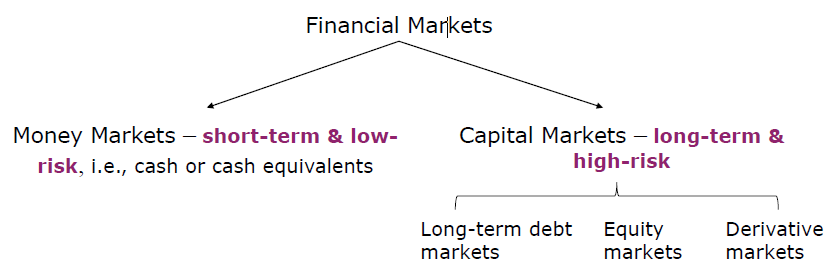
\includegraphics{Resources/Financialmarkets.png}

\hypertarget{money-markets}{%
\subsection{Money Markets}\label{money-markets}}

\begin{itemize}
\tightlist
\item
  Treasury bills
\item
  Certificates of Deposits (Term Deposits)
\item
  Commercial Paper(CP) (short term \textless{} 12month unsecured debts)
\item
  Bankers Acceptances (a postdated check, A bank, rather than an account holder, guarantees the payment.)
\item
  Eurodollars (U.S. dollar denominated deposits at foreign banks or foreign branches of U.S. banks)
\item
  Repurchase Agreements (Repos or RPs) and Reverse Repos.
\item
  Others, e.g., Brokers' Calls (interests charged by banks on loans made to brokerage firms), Federal Funds, The LIBOR Market, and Money Market Funds
\end{itemize}

\hypertarget{the-bond-market}{%
\subsection{The Bond Market}\label{the-bond-market}}

\begin{itemize}
\tightlist
\item
  Treasury Notes/Bonds (\$21 billion, \$21/\$51= 41\% of 2020 US Bond Market)
\item
  Mortgages and Mortgage Backed Securities (\$12.7 billion, 25\%
\item
  Corporate Bonds, including secured bonds, debentures (unsecured), callable/puttable/convertible bonds (\$10.6 billion, 21\%
\item
  Municipal Bonds (Issued by states/local, tax exempt) (\$3.95 billion, 7.8\%)
\item
  Federal Agency Debt, e.g., Fannie Mae, Freddie Mac ( 3.3\%)
\item
  International Bonds

  \begin{itemize}
  \tightlist
  \item
    Eurobonds: Eurodollar bonds bonds denominated in a currency other than the issuer's currency
  \item
    Yankee bond: US dollar denominated bond sold in the U.S. by a non U.S. issuer
  \end{itemize}
\item
  Inflation Protected Bonds (i.e., principal is adjusted per CPI)
\end{itemize}

\hypertarget{the-equity-market}{%
\subsection{The Equity Market}\label{the-equity-market}}

\begin{itemize}
\tightlist
\item
  Common stocks
\item
  Preferred stocks (pay preferred dividends, behaving like bond)
\item
  Depository receipts, (shares in a foreign company)

  \begin{itemize}
  \tightlist
  \item
    ADR American Depository Receipt
  \item
    CRD Chinese Depository receipt
  \item
    Reduced currency and foreign operation cost
  \end{itemize}
\end{itemize}

\hypertarget{market-indexes}{%
\subsection{Market Indexes}\label{market-indexes}}

\begin{itemize}
\tightlist
\item
  Broad based index (S\&P 500 etc.)
\item
  Narrow based index (composed of only a few stocks, in a specific industry)
\item
  Why indexes?
\item
  Provide performance benchmarks
\item
  Base of derivatives
\item
  Smart beta
\end{itemize}

The goal of \textbf{Smart beta} is to obtain alpha, lower risk or increase diversification at a cost lower than traditional active management and marginally higher than straight index investing

Construction Methodology

\begin{itemize}
\tightlist
\item
  Price weighted (DJIA) 1 share per firm
\item
  Market value weighted (S\&P500, NASDAQ)
\item
  Equal weighted (simple average of returns)
\end{itemize}

\hypertarget{derivative-markets}{%
\subsection{Derivative Markets}\label{derivative-markets}}

\begin{itemize}
\tightlist
\item
  A security with a pay-off that depends on the prices of other securities
\item
  Call/put options
\item
  Futures/Forwards
\item
  Swaps, futures options, etc.
\end{itemize}

Why we need them?

\begin{itemize}
\tightlist
\item
  Speculative
\item
  Hedging
\item
  Arbitraging (to lock in price)
\end{itemize}

\textbf{Arbitrage} describes the act of buying a security in one market and simultaneously selling it in another market at a higher price, thereby enabling investors to profit from the temporary difference in cost per share.

\hypertarget{securities-markets-and-trading}{%
\section{Securities Markets and Trading}\label{securities-markets-and-trading}}

Originators

\begin{itemize}
\tightlist
\item
  Publicly traded companies initial public offering (IPO), and seasonal equity offerings (SEOs), - Privately held firms (private placement in which shares are sold directly to
  a small group of institutional or wealthy investors)
\item
  Shelf registrations (public firms can register securities and gradually sell them to the public )
\end{itemize}

How securities are traded (in secondary markets)

\begin{itemize}
\tightlist
\item
  Direct search (e.g.~painting)
\item
  Brokered
\item
  Dealer
\item
  Auctions
\end{itemize}

ype of orders
maket order
price contingeant order

Trading mechanisms
OTC dealer
electronic
market maker (increase liquidity)
--
Over the counter dealer markets (OTC Markets)
-
Electronic communication networks ( ECNs)

margin trading

why to purchase with margin?

able to make more profits by borrowing money from broker, essentially multiplying market fluctuation/volatility.

short sale (borrow stocks to sell and payback when you sold it at profit)

derivative market (sell, not borrowing)

\hypertarget{market-participants}{%
\section{Market Participants}\label{market-participants}}

\hypertarget{investment-company}{%
\subsection{Investment company}\label{investment-company}}

\begin{itemize}
\tightlist
\item
  Intermediary that invest for investors
\item
  Record and admin
\item
  professional management
\item
  Lower transaction cost by volume
\end{itemize}

Net Asset Value (NAV)

\[\frac{Asset - Liabilities}{share outstanding}\]
unit investement fund (unmanaged) fixed portfolio for life

Managed Investment companies
- open-end(publicly trader and closed ended)
- close end funds shares sold at discount for liquidity (to sell quickly)

Exchange Traded Funds (ETF)

Can be continuously traded like stocks

Other Comingled Funds, Real Estate Investment Trusts, Hedged Funds

Mutual Funds 65\% of market

\begin{itemize}
\tightlist
\item
  Money market
\item
  equity funds (income vs growth)
\item
  specialised
\item
  bond
\item
  index funds
\item
  Funds of Funds
\end{itemize}

Funds can be sold directly, indirectly and through financial supermarkets

Fee structure

\begin{itemize}
\tightlist
\item
  Operating expense
\item
  front end load
\item
  back end load
\item
  12b-1 charges annual fee fro marketing and distribution
\end{itemize}

fee structure is very important and made large apart of your profit share

Taxation

no tax at fund level
long term capital gain tax rate
high turnover rate

ETF
- Passive investement, track index
- lower cost
- smart beta fund

\begin{itemize}
\tightlist
\item
  Bid ask spread (depend on demand)
\item
  Index price depart from NAV
\end{itemize}

mutual fund underperformed passive funds(cost of high freq trading)

consistent performance, don't be obsessed with top performer, they could be winner by chance

\hypertarget{ch2}{%
\chapter{Risk and Return}\label{ch2}}

\hypertarget{learning-objectives}{%
\section{Learning Objectives}\label{learning-objectives}}

This lecture aims to provide the ability to:

\begin{enumerate}
\def\labelenumi{\arabic{enumi}.}
\tightlist
\item
  Compute various measures of return on multi-year investments.
\item
  Determine the expected return and risk of portfolios combining risky assets and risk-free investments like Treasury bills.
\item
  Use the \textbf{Sharpe ratio} for evaluating portfolio performance and guiding capital allocation.
\item
  Understand the role of utility in determining optimal capital allocation to risky assets.
\end{enumerate}

\hypertarget{measuring-returns}{%
\section{Measuring Returns}\label{measuring-returns}}

Returns can be measured in several ways:

\begin{itemize}
\tightlist
\item
  \textbf{Holding Period Return (HPR):} This is the return earned over the period an investment is held.
\item
  \textbf{Returns Over Multiple Periods:} These can be compounded over time using methods such as:

  \begin{itemize}
  \tightlist
  \item
    arithmetic average,
  \item
    geometric average (compound annual growth rate), and
  \item
    dollar-weighted average (internal rate of return).
  \end{itemize}
\end{itemize}

\hypertarget{arithmetic-average}{%
\subsection{Arithmetic Average}\label{arithmetic-average}}

\[ \text{Arithmetic Average} = \frac{1}{N} \sum_{i=1}^{N} r_i \]
where \(r_i\) is the return in period \(i\) and \(N\) is the total number of periods.

\hypertarget{geometric-average}{%
\subsection{Geometric Average}\label{geometric-average}}

\[ \text{Geometric Average} = \left( \prod_{i=1}^{N} (1 + r_i) \right)^{\frac{1}{N}} - 1 \]

where \(r_i\) is the return in period \(i\) and \(N\) is the total number of periods.

\hypertarget{dollar-weighted-average-internal-rate-of-return}{%
\subsection{Dollar-Weighted Average (Internal Rate of Return)}\label{dollar-weighted-average-internal-rate-of-return}}

The dollar-weighted average return, or internal rate of return (IRR), is the discount rate \(r\) that sets the \textbf{net present value (NPV) = 0}. It is calculated by solving the following equation:

\[ \text{Dollar-Weighted Average} = \sum_{t=0}^{N} \frac{C_t}{(1 + r)^t} = 0 \]

Where \(C_t\) is the net cash flow at time \(t\), and \(N\) is the total number of periods.

\hypertarget{annualizing-returns}{%
\subsection{Annualizing Returns}\label{annualizing-returns}}

\begin{itemize}
\tightlist
\item
  \textbf{Annual Percentage Rate (APR):} Simple annualized interest rate without compounding.
\item
  \textbf{Effective Annual Rate (EAR):} Accounts for intra-year compounding, providing a true measure of annual return.
\end{itemize}

\[
\text{APR} = r \times n
\]

Where:

\begin{itemize}
\tightlist
\item
  \(r\) is the periodic interest rate
\item
  \(n\) is the number of compounding periods per year
\end{itemize}

\[
\text{EAR} = \left(1 + \frac{r}{n}\right)^n - 1
\]
Where:

\begin{itemize}
\tightlist
\item
  \(r\) is the nominal annual interest rate
\item
  \(n\) is the number of compounding periods per year
\end{itemize}

Example:

\$ 10000 Deposit, APR (annual percentage rate): 4\% p.a. Compounding Quarterly.

\[ 
\begin{aligned}
EAR &= (1+r/n)^n− 1 \\
&=(1+(0.04)/4)^4 −1 \\
&=0.0406 \\
&= 4.06\% 
\end{aligned}
\]

\hypertarget{risk-and-risk-premiums}{%
\section{Risk and Risk Premiums}\label{risk-and-risk-premiums}}

\hypertarget{expected-return}{%
\subsection{Expected Return}\label{expected-return}}

\(E(R)\) Is the weighted average of all possible returns, with weights being the probabilities of each scenario.

\[
E(R) = \sum_{i=1}^{N} p_i \cdot r_i
\]
Where:

\begin{itemize}
\tightlist
\item
  \(E(R)\) is the expected return of the portfolio
\item
  \(p_i\) is the probability/weight of asset \(i\) in the portfolio
\item
  \(r_i\) is the expected return of individual asset \(i\)
\item
  \(N\) is the number of assets in the portfolio
\end{itemize}

\textbf{Example Calculation}

\begin{itemize}
\tightlist
\item
  Asset A: weight = 50\%, expected return = 10\%
\item
  Asset B: weight = 30\%, expected return = 15\%
\item
  Asset C: weight = 20\%, expected return = 20\%
\end{itemize}

The expected return of the portfolio is:

\[
\begin{aligned}
E(R) &= (0.50 \cdot 0.10) + (0.30 \cdot 0.15) + (0.20 \cdot 0.20) \\
       &= 0.05 + 0.045 + 0.04 \\
       &= 0.135 \\
       &= 13.5\% \\  
\end{aligned}
\]
\textbf{R Code for Calculation}

\begin{Shaded}
\begin{Highlighting}[]
\CommentTok{\# Define the weights and expected returns of the assets}
\NormalTok{weights          }\OtherTok{\textless{}{-}} \FunctionTok{c}\NormalTok{(}\FloatTok{0.50}\NormalTok{, }\FloatTok{0.30}\NormalTok{, }\FloatTok{0.20}\NormalTok{)}
\NormalTok{expected\_returns }\OtherTok{\textless{}{-}} \FunctionTok{c}\NormalTok{(}\FloatTok{0.10}\NormalTok{, }\FloatTok{0.15}\NormalTok{, }\FloatTok{0.20}\NormalTok{)}

\CommentTok{\# Calculate the expected return of the portfolio}
\NormalTok{expected\_return\_portfolio }\OtherTok{\textless{}{-}} \FunctionTok{sum}\NormalTok{(weights }\SpecialCharTok{*}\NormalTok{ expected\_returns)}

\CommentTok{\# Print the expected return as a percentage}
\NormalTok{expected\_return\_percentage }\OtherTok{\textless{}{-}}\NormalTok{ expected\_return\_portfolio }\SpecialCharTok{*} \DecValTok{100}
\NormalTok{expected\_return\_percentage}
\end{Highlighting}
\end{Shaded}

\begin{verbatim}
## [1] 13.5
\end{verbatim}

\hypertarget{standard-deviation}{%
\subsection{Standard Deviation}\label{standard-deviation}}

Measures the deviation of returns from the mean.

\[
\sigma = \sqrt{\sum_{i=1}^{N} p(i) [r(i) - E(r)]^2}
\]

Where:

\begin{itemize}
\tightlist
\item
  \(\sigma\) is the standard deviation of the expected return
\item
  \(p(i)\) is the probability/weight of assets \(i\)
\item
  \(r(i)\) is the return of individual assets \(i\)
\item
  \(E(r)\) is the expected return
\item
  \(N\) is the number of assets
\end{itemize}

\textbf{Example Calculation}

\begin{itemize}
\tightlist
\item
  asset 1: probability = 0.3, return = 0.12
\item
  asset 2: probability = 0.4, return = 0.04
\item
  asset 3: probability = 0.3, return = -0.02
\item
  Expected return \(E(r) = 0.046\)
\end{itemize}

The standard deviation of the expected return is:

\[
\begin{aligned}
\sigma &= \sqrt{0.3(0.12 - 0.046)^2 + 0.4(0.04 - 0.046)^2 + 0.3(-0.02 - 0.046)^2}\\
       &= 0.0544\\
       &= 5.44\%
\end{aligned}
\]
\textbf{R Code for Calculation}

\begin{Shaded}
\begin{Highlighting}[]
\CommentTok{\# Define the probabilities and returns of the states}
\NormalTok{probabilities }\OtherTok{\textless{}{-}} \FunctionTok{c}\NormalTok{(}\FloatTok{0.3}\NormalTok{, }\FloatTok{0.4}\NormalTok{, }\FloatTok{0.3}\NormalTok{)}
\NormalTok{returns }\OtherTok{\textless{}{-}} \FunctionTok{c}\NormalTok{(}\FloatTok{0.12}\NormalTok{, }\FloatTok{0.04}\NormalTok{, }\SpecialCharTok{{-}}\FloatTok{0.02}\NormalTok{)}
\NormalTok{expected\_return }\OtherTok{\textless{}{-}} \FloatTok{0.046}

\CommentTok{\# Calculate the variance}
\NormalTok{variance }\OtherTok{\textless{}{-}} \FunctionTok{sum}\NormalTok{(probabilities }\SpecialCharTok{*}\NormalTok{ (returns }\SpecialCharTok{{-}}\NormalTok{ expected\_return)}\SpecialCharTok{\^{}}\DecValTok{2}\NormalTok{)}

\CommentTok{\# Calculate the standard deviation}
\NormalTok{standard\_deviation }\OtherTok{\textless{}{-}} \FunctionTok{sqrt}\NormalTok{(variance)}

\CommentTok{\# Print the standard deviation as a percentage}
\NormalTok{standard\_deviation\_percentage }\OtherTok{\textless{}{-}}\NormalTok{ standard\_deviation }\SpecialCharTok{*} \DecValTok{100}
\NormalTok{standard\_deviation\_percentage}
\end{Highlighting}
\end{Shaded}

\begin{verbatim}
## [1] 5.444263
\end{verbatim}

\hypertarget{normal-distribution}{%
\subsection{Normal Distribution}\label{normal-distribution}}

Stock returns are often assumed to be normally distributed. However, real return distributions may show skewness such as ``fat tails.''

\[X∼N(μ,σ2)\]

\[
f(x | \mu, \sigma) = \frac{1}{\sigma \sqrt{2\pi}} \exp\left(-\frac{(x - \mu)^2}{2\sigma^2}\right)
\]

Where:

\begin{itemize}
\tightlist
\item
  \(\mu\) is the mean
\item
  \(\sigma\) is the standard deviation
\item
  \(x\) is the variable
\end{itemize}

\textbf{standard normal distribution} is the normal distribution with mean \(μ\) = 0 and standard deviation \(σ\) = 1.

\[
f(x) = \frac{1}{\sqrt{2\pi}} \exp\left(-\frac{x^2}{2}\right)
\]

Where:

\begin{itemize}
\tightlist
\item
  \(\mu = 0\)
\item
  \(\sigma = 1\)
\item
  \(x\) is the variable
\end{itemize}

\textbf{Example Calculation}

Let's calculate the probability of a value \(x\) in a normal distribution with a mean \(\mu = 0\) and a standard deviation \(\sigma = 1\) (standard normal distribution).

We will also calculate the cumulative probability (CDF) and quantiles for specific values.

\textbf{R Code for Calculation}

\begin{Shaded}
\begin{Highlighting}[]
\CommentTok{\# Define the parameters for the normal distribution}
\NormalTok{mu }\OtherTok{\textless{}{-}} \DecValTok{0}
\NormalTok{sigma }\OtherTok{\textless{}{-}} \DecValTok{1}

\CommentTok{\# Define a value for x}
\NormalTok{x }\OtherTok{\textless{}{-}} \DecValTok{1}

\CommentTok{\# Calculate the probability density function (PDF) of the normal distribution at x}
\NormalTok{pdf\_value }\OtherTok{\textless{}{-}} \FunctionTok{dnorm}\NormalTok{(x, }\AttributeTok{mean =}\NormalTok{ mu, }\AttributeTok{sd =}\NormalTok{ sigma)}

\CommentTok{\# Calculate the cumulative distribution function (CDF) of the normal distribution at x}
\NormalTok{cdf\_value }\OtherTok{\textless{}{-}} \FunctionTok{pnorm}\NormalTok{(x, }\AttributeTok{mean =}\NormalTok{ mu, }\AttributeTok{sd =}\NormalTok{ sigma)}

\CommentTok{\# Calculate the quantile for a given probability}
\NormalTok{probability }\OtherTok{\textless{}{-}} \FloatTok{0.95}
\NormalTok{quantile\_value }\OtherTok{\textless{}{-}} \FunctionTok{qnorm}\NormalTok{(probability, }\AttributeTok{mean =}\NormalTok{ mu, }\AttributeTok{sd =}\NormalTok{ sigma)}

\CommentTok{\# Print the results}
\FunctionTok{list}\NormalTok{(}\AttributeTok{PDF =}\NormalTok{ pdf\_value, }\AttributeTok{CDF =}\NormalTok{ cdf\_value, }\AttributeTok{Quantile =}\NormalTok{ quantile\_value)}
\end{Highlighting}
\end{Shaded}

\begin{verbatim}
## $PDF
## [1] 0.2419707
## 
## $CDF
## [1] 0.8413447
## 
## $Quantile
## [1] 1.644854
\end{verbatim}

\hypertarget{risk-aversion}{%
\subsection{Risk Aversion}\label{risk-aversion}}

Risk-averse investors prefer less risk for the same expected return. They demand a risk premium for taking additional risk, quantified by the price of risk (ratio of risk premium to variance).

Risk-averse investors reject investment opportunities with a \textbf{risk premium} of zero or less.

\textbf{Degree of risk aversion}

\[
A = \frac{E(r_i) - E(r_f)}{\sigma_i^2}
\]

Where:

\begin{itemize}
\tightlist
\item
  \(A\) = degree of risk aversion
\item
  \(E(r_i)\) is the expected return of the risky asset.
\item
  \(E(r_f)\) is the risk-free rate.
\item
  \(\sigma_i^2\) is the variance of the return of the risky asset.
\end{itemize}

\textbf{Example}

For the market portfolio (e.g., S\&P 500 index funds), the average degree of risk aversion of investors is:

\[
\begin{aligned}
\bar{A} &= \frac{\text{Average}(r_M - r_f)}{\text{Sample } \sigma_M^2}\\
 &\approx \frac{0.08}{0.04} = 2
\end{aligned}
\]

Where:

\begin{itemize}
\tightlist
\item
  \(r_M\) is the return of the market portfolio.
\item
  \(\sigma_M^2\) is the variance of the market return.
\end{itemize}

\hypertarget{portfolio-construction}{%
\section{Portfolio Construction}\label{portfolio-construction}}

\begin{enumerate}
\def\labelenumi{\arabic{enumi}.}
\item
  Selection of risky assets/portfolios such as stocks and bonds.
\item
  Decision on the proportion of the portfolio to invest in risky assets versus risk-free assets.
\end{enumerate}

\hypertarget{capital-allocation}{%
\subsection{Capital Allocation:}\label{capital-allocation}}

Combining investments in risk-free and risky assets allows for varying expected returns and risks.

We call the overall portfolio composed of the risk-free asset and the risky portfolio the \textbf{complete portfolio}.

\hypertarget{utility}{%
\subsection{Utility}\label{utility}}

\textbf{Utility:} Represents investor preferences, considering risk aversion. It helps in making decisions about different securities.This is a single measure we have the investor's attitudes to risk and return at each level of wealth.

\textbf{Influence of the trade-off decisions:}

\begin{itemize}
\tightlist
\item
  Risk appetite (strong financial position and stable income may have higher appitite)
\item
  proportion of the investor's total wealth. (psychological risk aversion)
\item
  Financial Goals/liquidity needs (set when they need cash flow)
\item
  Investment Horizon (longer horizon takes more risk)
\item
  Knowledge and Experience (Dunning Kruger effect)
\item
  Social/Regulatory environment and incentives
\end{itemize}

\hypertarget{utility-function}{%
\subsection{Utility Function}\label{utility-function}}

Captures an investor's risk-return trade-offs. Utility increases with expected return and decreases with risk. More risk-averse investors have higher coefficients of risk aversion (A).

There are countless utility functions. An example is:

\[
U = E(r) - \frac{1}{2} A \sigma^2
\]
Where:

\begin{itemize}
\tightlist
\item
  \(U\) = the utility value,
\item
  \(A\) = coefficient of risk aversion,
\item
  \(\sigma^2\) = variance
\item
  Utility increases with expected returns and decreases with risk.
\item
  Utility of a risk-free portfolio is equal to its rate of return.
\item
  More risk-averse investors will have larger values of A.
\item
  Investors assign higher utility to more attractive risk-return portfolios.
\end{itemize}

\textbf{Example:}

where:

\begin{itemize}
\tightlist
\item
  \(A\) degree of risk aversion = \(2\)
\item
  \(r_f\) risk-free rate = \(4\%\)
\end{itemize}

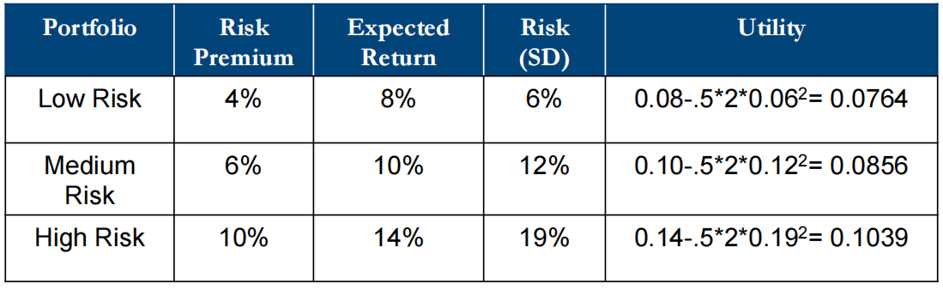
\includegraphics{Resources/utilisation.png}

\hypertarget{indifference-curves}{%
\subsection{Indifference Curves}\label{indifference-curves}}

These curves connect portfolios providing the same utility level, illustrating an investor's preference for different risk-return combinations.

Simply above the curve Yes, below the curve no.

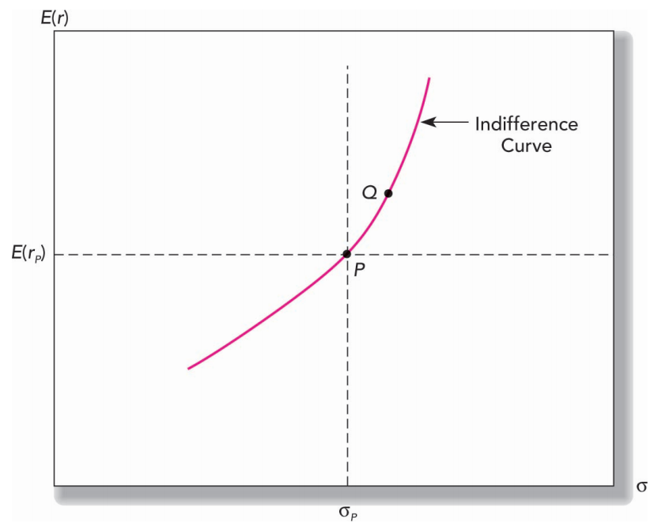
\includegraphics{Resources/indiffcurve.png}

\hypertarget{capital-allocation-line}{%
\subsection{Capital Allocation Line}\label{capital-allocation-line}}

It's possible to split investment funds between safe and risky assets.

\begin{enumerate}
\def\labelenumi{\arabic{enumi}.}
\tightlist
\item
  Risk free asset: proxy = T-bills
\item
  Risky asset: stock (or a portfolio)
\end{enumerate}

\begin{itemize}
\tightlist
\item
  \(r_f\) Risk-free rate = \(7\%\)
\item
  \(\sigma_{r_f}\) Standard deviation of the risk-free rate = \(0\)
\item
  \(E(r_p)\) Expected return of the risky portfolio = \(15\%\)
\item
  \(\sigma_p\) Standard deviation of the risky portfolio = \(22\%\)
\end{itemize}

The investor allocates \(y\) proportion of their wealth in the risky portfolio and \(1 - y\) in the risk-free portfolio.

\[
\begin{aligned}
E(r_c) &= (y)E(r_p) + (1 - y)r_f \\
E(r_c) &= y \times 15\% + (1 - y) \times 7\% \\
E(r_c) &= 7\% + y \times (15\% - 7\%) \\
E(r_c) &= 7\% + 8y \\
and \\
\sigma_c &= y \sigma_𝑝=22𝑦\\
\end{aligned}
\]

Example:

\[
\begin{aligned}
y        &= 0.75 \\
r_𝑐     &= 0.07+0.08*(0.75) = 13\% \\
\sigma_c &= y \sigma_𝑝=22𝑦\\
\sigma_c &= 16.5\% \\
\end{aligned}
\]
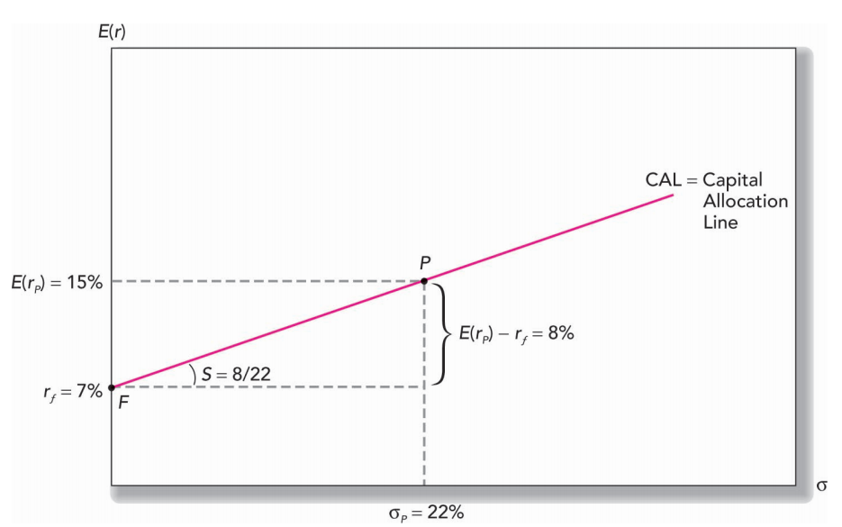
\includegraphics{Resources/capaloocation1.png}

The \textbf{Sharpe Ratio}, which measures extra return per unit of risk (gradient of line), is calculated as:

\[
\begin{aligned}
\text{Sharpe ratio} &= \frac{E(r_p) - r_f}{ \sigma_p}\\
&= 8/22 \\
&= 0.36\%. 
\end{aligned}
\]

\hypertarget{capital-allocation-line-cal-with-leverage}{%
\subsection{Capital Allocation Line (CAL) with Leverage}\label{capital-allocation-line-cal-with-leverage}}

Leverage multiplies loss and return at a cost of borrowing money from dealers.

Borrowing at the risk-free rate extends the CAL. Borrowing rates higher than the risk-free rate cause a kink in the CAL, changing the slope.

\[
\begin{aligned}
      𝐸(r_c) &= (−0.5)∗0.09+(1.5)∗0.15\\
              &=18\% \\
       \sigma_c &= (1.5)0.22 = 33\% \\
\text{The Sharpe ratio is} \\
    (18−9)/0.33 &= 0.27\% \\
\end{aligned}
\]
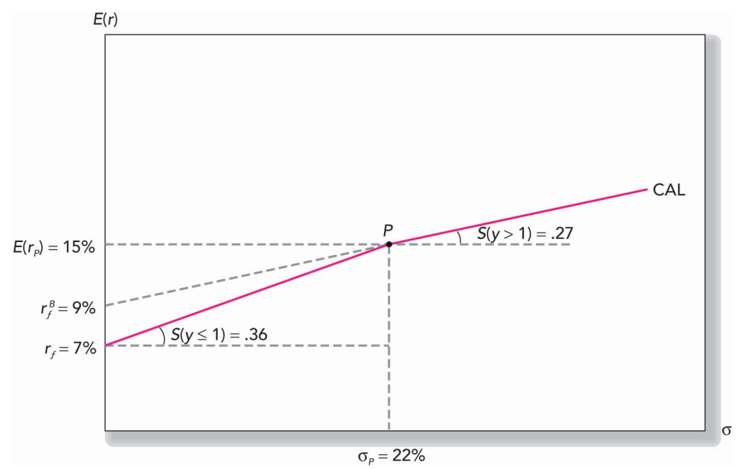
\includegraphics{Resources/capaloocation2.png}

\hypertarget{utility-maximization}{%
\subsection{Utility Maximization}\label{utility-maximization}}

In portfolio theory, investors aim to maximize their utility, which balances expected return and risk. Mathematically, the utility function is:

\[
\begin{aligned}
\text{Max}(U) &= E(r) - \frac{1}{2} A \sigma^2 \\
&= r_f + y [E(r_p) - r_f] - \frac{1}{2} A y^2 \sigma_p^2 \\
\text{Solve for y, we have } \\
y^* &= \frac{E(r_p) - r_f}{A \sigma_p^2}
\end{aligned}
\]

To find the optimal proportion \(y^\) to invest in the risky portfolio, we solve for \(y_*\):

\textbf{R code}

\begin{Shaded}
\begin{Highlighting}[]
\CommentTok{\# Define parameters}
\NormalTok{rf }\OtherTok{\textless{}{-}} \FloatTok{0.06}       \CommentTok{\# Risk{-}free rate}
\NormalTok{Erp }\OtherTok{\textless{}{-}} \FloatTok{0.18}      \CommentTok{\# Expected return of the risky portfolio}
\NormalTok{sigma\_p }\OtherTok{\textless{}{-}} \FloatTok{0.25}  \CommentTok{\# Standard deviation of the risky portfolio}
\NormalTok{A }\OtherTok{\textless{}{-}} \DecValTok{5}           \CommentTok{\# Degree of risk aversion}

\CommentTok{\# Calculate optimal y}
\NormalTok{y\_star }\OtherTok{\textless{}{-}}\NormalTok{ (Erp }\SpecialCharTok{{-}}\NormalTok{ rf) }\SpecialCharTok{/}\NormalTok{ (A }\SpecialCharTok{*}\NormalTok{ sigma\_p}\SpecialCharTok{\^{}}\DecValTok{2}\NormalTok{)}
\NormalTok{y\_star}
\end{Highlighting}
\end{Shaded}

\begin{verbatim}
## [1] 0.384
\end{verbatim}

\begin{Shaded}
\begin{Highlighting}[]
\CommentTok{\# The Expected Return}

\NormalTok{ER }\OtherTok{=}\NormalTok{ rf }\SpecialCharTok{+}\NormalTok{ (y\_star}\SpecialCharTok{*}\NormalTok{(Erp }\SpecialCharTok{{-}}\NormalTok{ rf))}
\NormalTok{ER}
\end{Highlighting}
\end{Shaded}

\begin{verbatim}
## [1] 0.10608
\end{verbatim}

\begin{Shaded}
\begin{Highlighting}[]
\NormalTok{sigma\_c }\OtherTok{=}\NormalTok{ y\_star}\SpecialCharTok{*}\NormalTok{sigma\_p}
\NormalTok{sigma\_c}
\end{Highlighting}
\end{Shaded}

\begin{verbatim}
## [1] 0.096
\end{verbatim}

\begin{Shaded}
\begin{Highlighting}[]
\NormalTok{sharpe }\OtherTok{=}\NormalTok{ (ER}\SpecialCharTok{{-}}\NormalTok{ rf)}\SpecialCharTok{/}\NormalTok{sigma\_c}
\NormalTok{sharpe}
\end{Highlighting}
\end{Shaded}

\begin{verbatim}
## [1] 0.48
\end{verbatim}

\hypertarget{personal-preferences}{%
\subsection{Personal preferences}\label{personal-preferences}}

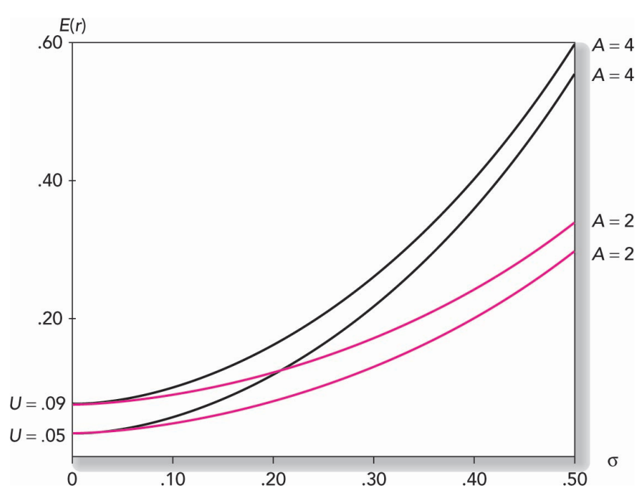
\includegraphics{Resources/capaloocation3.png}

\begin{itemize}
\tightlist
\item
  Investors aim to choose portfolios on higher indifference curves.
\item
  Higher indifference curves provide a higher expected return for a given level of risk.
\item
  More risk-averse investors have steeper indifference curves.
\item
  More risk-averse investors require a greater increase in expected return for an increase in portfolio risk.
\end{itemize}

\hypertarget{the-capital-market-line-cml}{%
\subsection{The Capital Market Line (CML)}\label{the-capital-market-line-cml}}

\begin{longtable}[]{@{}
  >{\raggedright\arraybackslash}p{(\columnwidth - 4\tabcolsep) * \real{0.1829}}
  >{\raggedright\arraybackslash}p{(\columnwidth - 4\tabcolsep) * \real{0.4268}}
  >{\raggedright\arraybackslash}p{(\columnwidth - 4\tabcolsep) * \real{0.3902}}@{}}
\toprule\noalign{}
\begin{minipage}[b]{\linewidth}\raggedright
\textbf{Aspect}
\end{minipage} & \begin{minipage}[b]{\linewidth}\raggedright
\textbf{Active Management}
\end{minipage} & \begin{minipage}[b]{\linewidth}\raggedright
\textbf{Passive Management}
\end{minipage} \\
\midrule\noalign{}
\endhead
\bottomrule\noalign{}
\endlastfoot
\textbf{Pros} & & \\
Higher Return Potential & Aims to outperform the market. & Matches market returns. \\
Flexibility & Can quickly adjust to market changes. & Follows index rules. \\
Risk Management & Can avoid certain sectors or stocks to manage risk. & Diversified holdings reduce specific risks. \\
Exploiting Inefficiencies & Can capitalize on market inefficiencies. & Benefits from overall market growth. \\
Customization & Tailors strategy to investor goals. & Simple, straightforward strategy. \\
\textbf{Cons} & & \\
Higher Costs & More fees and expenses due to frequent trading and research. & Lower fees and expenses. \\
Performance Uncertainty & No guarantee of outperforming the market. & Predictable performance, matches index. \\
Increased Risk & Higher risk from concentrated positions and market timing. & Lower risk due to diversification. \\
Tax Implications & More frequent trading can lead to higher taxes. & Less frequent trading, more tax efficient. \\
Dependence on Manager Skill & Relies on the skill and judgment of the manager. & No reliance on manager skill. \\
\end{longtable}

\hypertarget{ch3}{%
\chapter{Diversification}\label{ch3}}

\hypertarget{portfolio-construction-1}{%
\subsection{Portfolio Construction}\label{portfolio-construction-1}}

Portfolio construction generally has three steps:

\begin{enumerate}
\def\labelenumi{\arabic{enumi}.}
\tightlist
\item
  \textbf{Capital allocation} between the risky portfolio and risk-free assets
\item
  \textbf{Asset allocation} across wide asset classes (stocks, international stocks, long-term bonds).
\item
  \textbf{Security selection}.
\end{enumerate}

\hypertarget{major-risks-of-stock-portfolio}{%
\section{Major Risks of Stock Portfolio}\label{major-risks-of-stock-portfolio}}

\begin{longtable}[]{@{}
  >{\raggedright\arraybackslash}p{(\columnwidth - 2\tabcolsep) * \real{0.2687}}
  >{\raggedright\arraybackslash}p{(\columnwidth - 2\tabcolsep) * \real{0.7313}}@{}}
\toprule\noalign{}
\begin{minipage}[b]{\linewidth}\raggedright
Risk Type
\end{minipage} & \begin{minipage}[b]{\linewidth}\raggedright
Description
\end{minipage} \\
\midrule\noalign{}
\endhead
\bottomrule\noalign{}
\endlastfoot
\textbf{Market Risk} & Fluctuations in overall market affecting portfolio value. \\
Sector Risk & Specific sectors or industries under-performing. \\
\textbf{Company Risk} & Individual companies facing financial difficulties or poor performance. \\
Liquidity Risk & Difficulty in buying or selling assets without significant price changes. \\
Currency Risk & Exchange rate fluctuations impacting international investments. \\
Interest Rate Risk & Changes in interest rates affecting bond prices and portfolio value. \\
Political Risk & Political events or policy changes impacting financial markets. \\
Regulatory Risk & Changes in regulations affecting industries or companies in the portfolio. \\
\end{longtable}

\begin{itemize}
\tightlist
\item
  Market risk (\textbf{systematic risk}): non-diversifiable risk
\item
  Unique risk (\textbf{non-systematic risk}): firm-specific risk, diversifiable risk
\end{itemize}

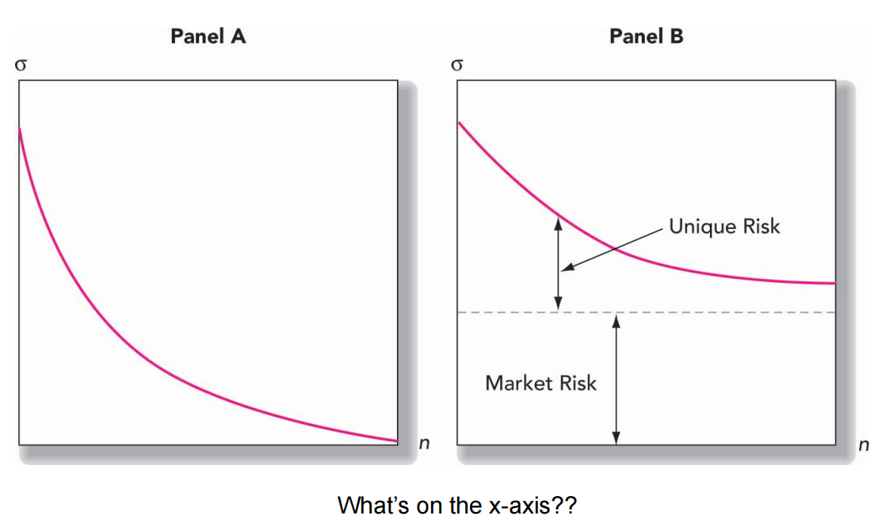
\includegraphics{Resources/sysrisk.png}

\hypertarget{portfolio-calculations}{%
\section{Portfolio Calculations}\label{portfolio-calculations}}

\hypertarget{expected-return-1}{%
\subsection{Expected return}\label{expected-return-1}}

The \textbf{expected return} of the portfolio is

\[ E(r_P) = w_1 E(r_1) + w_2 E(r_2) \]

Where:

\begin{itemize}
\tightlist
\item
  \(E(r_P)\)is the expected return of the portfolio.
\item
  \(w_1\) is the weight of asset 1 in the portfolio.
\item
  \(E(r_1)\) is the expected return of asset 1.
\item
  \(w_2\) is the weight of asset 2 in the portfolio.
\item
  \(E(r_2)\) is the expected return of asset 2.
\end{itemize}

\hypertarget{variance}{%
\subsection{variance}\label{variance}}

\textbf{Variance} measures how much the values of a random variable vary or spread out from the mean (average)

The \textbf{variance} of the portfolio \(\sigma_P^2\) can be calculated using the following formula:

\[ \sigma_P^2 = w_1^2 \sigma_1^2 + w_2^2 \sigma_2^2 + 2w_1 w_2 \rho_{12} \sigma_1 \sigma_2 \]

Where:

\begin{itemize}
\tightlist
\item
  \(\sigma_P^2\) is the variance of the portfolio.
\item
  \(w_1\) is the weight of asset 1 in the portfolio.
\item
  \(\sigma_1^2\) is the variance of returns of asset 1.
\item
  \$w\_2 \$ is the weight of asset 2 in the portfolio.
\item
  \(\sigma_2^2\) is the variance of returns of asset 2.
\item
  \(\rho_{12}\) is the correlation coefficient between returns of assets 1 and 2.
\item
  \(\sigma_1\) and \(\sigma_2\) are the standard deviations of returns of assets 1 and 2, respectively.
\end{itemize}

The variance formula accounts for the individual variances of assets 1 and 2, as well as their \textbf{covariance}.

\[Cov(r_1,r_2 )=\rho_{12} 𝜎_1 𝜎_2\]

\hypertarget{case-i-1}{%
\subsubsection{\texorpdfstring{Case I: \$ \rho = 1 \$}{Case I: \$ = 1 \$}}\label{case-i-1}}

When the correlation coefficient is 1, the formula simplifies to:

\[
\begin{aligned}
\sigma_P^2 &= (w_1 \sigma_1 + w_2 \sigma_2)^2 \\
\sigma_P  &= w_1 \sigma_1 + w_2 \sigma_2 \\
\end{aligned}
\]

\hypertarget{case-ii--1}{%
\subsubsection{\texorpdfstring{Case II: \$ \rho = -1 \$}{Case II: \$ = -1 \$}}\label{case-ii--1}}

When the correlation coefficient is -1, the formula simplifies to:

\[
\begin{aligned}
\sigma_P^2 &= (w_1 \sigma_1 - w_2 \sigma_2)^2 \\
\sigma_P  &= w_1 \sigma_1 - w_2 \sigma_2 \\
\end{aligned}
\]

\hypertarget{covariance}{%
\subsection{Covariance}\label{covariance}}

The \textbf{covariance} between returns of assets A and B (\(Cov(r_A, r_B)\)) can be calculated using the following formula:

\[Cov(r_A, r_B) = \sum_{i=1}^{n} p(i)[r_A(i) - E(r_A)][r_B(i) - E(r_B)]\]

Where:

\begin{itemize}
\tightlist
\item
  \(Cov(r_A, r_B)\) is the covariance between returns of assets A and B.
\item
  \(p(i)\) is the probability of scenario \(i\).
\item
  \(r_A(i)\) and \(r_B(i)\) are the returns of assets A and B, respectively, in scenario \(i\).
\item
  \(E(r_A)\) and \(E(r_B)\) are the expected returns of assets A and B, respectively.
\end{itemize}

\textbf{R code}

\begin{Shaded}
\begin{Highlighting}[]
\NormalTok{returns\_A }\OtherTok{\textless{}{-}} \FunctionTok{c}\NormalTok{(}\FloatTok{0.05}\NormalTok{, }\FloatTok{0.03}\NormalTok{, }\FloatTok{0.02}\NormalTok{, }\FloatTok{0.06}\NormalTok{, }\FloatTok{0.04}\NormalTok{)  }\CommentTok{\# Returns for asset A}
\NormalTok{returns\_B }\OtherTok{\textless{}{-}} \FunctionTok{c}\NormalTok{(}\FloatTok{0.04}\NormalTok{, }\FloatTok{0.02}\NormalTok{, }\FloatTok{0.01}\NormalTok{, }\FloatTok{0.05}\NormalTok{, }\FloatTok{0.03}\NormalTok{)  }\CommentTok{\# Returns for asset B}

\CommentTok{\# Expected returns of assets A and B}
\NormalTok{E\_r\_A }\OtherTok{\textless{}{-}} \FunctionTok{mean}\NormalTok{(returns\_A)}
\NormalTok{E\_r\_B }\OtherTok{\textless{}{-}} \FunctionTok{mean}\NormalTok{(returns\_B)}

\CommentTok{\# Probabilities of scenarios}
\NormalTok{probabilities }\OtherTok{\textless{}{-}} \FunctionTok{c}\NormalTok{(}\FloatTok{0.2}\NormalTok{, }\FloatTok{0.15}\NormalTok{, }\FloatTok{0.25}\NormalTok{, }\FloatTok{0.1}\NormalTok{, }\FloatTok{0.3}\NormalTok{)}

\CommentTok{\# Calculation of covariance}
\NormalTok{covariance }\OtherTok{\textless{}{-}} \FunctionTok{sum}\NormalTok{(probabilities }\SpecialCharTok{*}\NormalTok{ (returns\_A }\SpecialCharTok{{-}}\NormalTok{ E\_r\_A) }\SpecialCharTok{*}\NormalTok{ (returns\_B }\SpecialCharTok{{-}}\NormalTok{ E\_r\_B))}

\CommentTok{\# Print the covariance}
\FunctionTok{print}\NormalTok{(}\FunctionTok{paste}\NormalTok{(}\StringTok{"Covariance between returns of assets A and B:"}\NormalTok{, covariance))}
\end{Highlighting}
\end{Shaded}

\begin{verbatim}
## [1] "Covariance between returns of assets A and B: 0.000175"
\end{verbatim}

\hypertarget{correlation}{%
\subsection{Correlation}\label{correlation}}

\[{\rho_12} = \frac{Cov(r_1,r_2 )}{\sigma_1 \sigma_2}\]

\begin{itemize}
\item
  The portfolio return is not affected by correlation between returns
\item
  Thus, investors should always prefer to add to their portfolios assets with low or negative correlation to diversify risks.
\end{itemize}

The lower the correlation, the greater the potential benefit from diversification.

\hypertarget{variance-calculations}{%
\subsection{Variance calculations}\label{variance-calculations}}

If we have perfectly negatively correlated assets in our portfolios, then the portfolio standard deviation can be reduced to zero by choosing appropriate weights.

Given:

\begin{itemize}
\tightlist
\item
  \(w_1\) = \(0.40\)
\item
  \(\sigma_1^2\) = \(0.014\)
\item
  \(w_2\) = \(0.60\)
\item
  \(\sigma_2^2\) = \(0.04\)
\item
  \(Cov(r_1, r_2)\) = \(0.0072\)
\end{itemize}

Calculate:
\[
\begin{aligned}
\rho        &= \frac{Cov(r_1, r_2)}{\sigma_1 \times \sigma_2} \\ 
            &= \frac{0.007}{\sqrt{0.014} \times \sqrt{0.04}} \\ 
            &= 0.3 \\
\end{aligned}
\]\\
\$\$

\begin{aligned}           
            
 \sigma_P^2 &= w_1^2 \sigma_1^2 + w_2^2 \sigma_2^2 + 2w_1 w_2 \rho(r_1, r_2) \sigma_1 \sigma_2 \\
            &= 0.40^2 (0.014) + 0.60^2 (0.04) + 2(0.40)(0.60)[0.3\sqrt{0.014} \times \sqrt{0.04}] \\
            &= 0.02 \\
\sigma_P    &= \sqrt{0.02} = 0.142 \\
\end{aligned}

\[            
\]

\begin{aligned} 

\text{Weighted}(\sigma) &= 0.40\sqrt{0.014} + 0.60\sqrt{0.04} \\
            &= 0.168 \\
            
\end{aligned}

\$\$

\[
\begin{aligned} 
\text{Diversification Benefit}
            &= 0.168 - 0.142 \\
            &= 0.026 
\end{aligned}
\]

\begin{Shaded}
\begin{Highlighting}[]
\CommentTok{\# Given values}
\NormalTok{w1 }\OtherTok{\textless{}{-}} \FloatTok{0.4}
\NormalTok{w2 }\OtherTok{\textless{}{-}} \FloatTok{0.6}
\NormalTok{sigma1\_squared }\OtherTok{\textless{}{-}} \FloatTok{0.014}
\NormalTok{sigma2\_squared }\OtherTok{\textless{}{-}} \FloatTok{0.04}
\NormalTok{covariance }\OtherTok{\textless{}{-}} \FloatTok{0.0072}

\CommentTok{\# Calculate correlation coefficient}
\NormalTok{rho }\OtherTok{\textless{}{-}}\NormalTok{ covariance }\SpecialCharTok{/} \FunctionTok{sqrt}\NormalTok{(sigma1\_squared }\SpecialCharTok{*}\NormalTok{ sigma2\_squared)}
\NormalTok{rho }
\end{Highlighting}
\end{Shaded}

\begin{verbatim}
## [1] 0.3042555
\end{verbatim}

\begin{Shaded}
\begin{Highlighting}[]
\CommentTok{\# Calculate portfolio variance}
\NormalTok{portfolio\_variance }\OtherTok{\textless{}{-}}\NormalTok{ w1}\SpecialCharTok{\^{}}\DecValTok{2} \SpecialCharTok{*}\NormalTok{ sigma1\_squared }\SpecialCharTok{+}\NormalTok{ w2}\SpecialCharTok{\^{}}\DecValTok{2} \SpecialCharTok{*}\NormalTok{ sigma2\_squared }\SpecialCharTok{+} \DecValTok{2} \SpecialCharTok{*}\NormalTok{ w1 }\SpecialCharTok{*}\NormalTok{ w2 }\SpecialCharTok{*}\NormalTok{ covariance}
\NormalTok{portfolio\_variance}
\end{Highlighting}
\end{Shaded}

\begin{verbatim}
## [1] 0.020096
\end{verbatim}

\begin{Shaded}
\begin{Highlighting}[]
\CommentTok{\# Calculate portfolio standard deviation}
\NormalTok{portfolio\_sd }\OtherTok{\textless{}{-}} \FunctionTok{sqrt}\NormalTok{(portfolio\_variance)}
\NormalTok{portfolio\_sd}
\end{Highlighting}
\end{Shaded}

\begin{verbatim}
## [1] 0.1417604
\end{verbatim}

\begin{Shaded}
\begin{Highlighting}[]
\CommentTok{\# Calculate weighted standard deviation}
\NormalTok{weighted\_sd }\OtherTok{\textless{}{-}}\NormalTok{ w1 }\SpecialCharTok{*} \FunctionTok{sqrt}\NormalTok{(sigma1\_squared) }\SpecialCharTok{+}\NormalTok{ w2 }\SpecialCharTok{*} \FunctionTok{sqrt}\NormalTok{(sigma2\_squared)}
\NormalTok{weighted\_sd}
\end{Highlighting}
\end{Shaded}

\begin{verbatim}
## [1] 0.1673286
\end{verbatim}

\begin{Shaded}
\begin{Highlighting}[]
\CommentTok{\# Calculate diversification benefit}
\NormalTok{diversification\_benefit }\OtherTok{\textless{}{-}}\NormalTok{ weighted\_sd }\SpecialCharTok{{-}}\NormalTok{ portfolio\_sd}
\NormalTok{diversification\_benefit}
\end{Highlighting}
\end{Shaded}

\begin{verbatim}
## [1] 0.02556828
\end{verbatim}

\hypertarget{risky-and-risk-free-assets}{%
\section{Risky and Risk-Free Assets}\label{risky-and-risk-free-assets}}

To decide the proportion of the portfolio to be allocated between the stock and bond funds, we will introduce a risk-free asset (T-bills) to the portfolio allocation problem.

\hypertarget{sharpe-ratio}{%
\subsection{Sharpe Ratio}\label{sharpe-ratio}}

The higher a fund's Sharpe ratio (Higher Return per Unit of Risk), the better its returns have been relative to the amount of investment risk taken.

\begin{longtable}[]{@{}ll@{}}
\toprule\noalign{}
Sharpe Ratio Range & Classification \\
\midrule\noalign{}
\endhead
\bottomrule\noalign{}
\endlastfoot
Less than 1 & Bad \\
1 to 1.99 & Adequate/Good \\
2 to 2.99 & Very Good \\
\end{longtable}

The objective function is to maximize:

\[\frac{{E(r_1) - r_f}}{{\sigma_P}}\]

where:

\[
\begin{aligned} 
E(r_1)    &= w_1 E(r_1) + w_2 E(r_2)\\
\sigma_P  &= \sqrt{{w_1^2 \sigma_1^2 + w_2^2 \sigma_2^2 + 2w_1 w_2 Cov(r_1, r_2)}}\\
\text{subject to}:\\
w_1 + w_2 &= 1\\
\end{aligned} 
\]

To solve for \(w_1\) and \(w_2\), we have:

\[
w_1 = \frac{{(E(r_1) - r_f) \sigma_2^2 - (E(r_2) - r_f) Cov(r_1, r_2)}}{{(E(r_1) - r_f) \sigma_2^2 + (E(r_2) - r_f) \sigma_1^2 - (E(r_1) - r_f + E(r_2) - r_f) Cov(r_1, r_2)}}$
$w_2 = 1 - w_1$
\]

Given:

\begin{itemize}
\tightlist
\item
  \(w_2 = 0.60\)
\item
  \(w_1 = 0.40\)
\end{itemize}

Thus,

\[
\begin{aligned} 
E(r_P)   &= 0.40 \times 8\% + 0.60 \times 13\% = 11\% \\
\sigma_P &= \sqrt{{0.40^2 \times 0.12^2 + 0.60^2 \times 0.20^2 + 2 \times 0.4 \times 0.6 \times (0.0072)}} \\ 
         &= 0.142 \\
\end{aligned}       
\]

\[
\begin{aligned} 
Sharpe \, ratio &= \frac{{E(r_P) - r_f}}{{\sigma_P}} \\
&= \frac{{0.11 - 0.03}}{{0.142}} \\
&= 0.42
\end{aligned} 
\]

\begin{Shaded}
\begin{Highlighting}[]
\CommentTok{\# Given values}
\NormalTok{w\_2 }\OtherTok{\textless{}{-}} \FloatTok{0.60}
\NormalTok{w\_1 }\OtherTok{\textless{}{-}} \FloatTok{0.40}
\NormalTok{r\_f }\OtherTok{\textless{}{-}} \FloatTok{0.03}
\NormalTok{E\_r\_1 }\OtherTok{\textless{}{-}} \FloatTok{0.08}
\NormalTok{E\_r\_2 }\OtherTok{\textless{}{-}} \FloatTok{0.13}
\NormalTok{sigma\_1 }\OtherTok{\textless{}{-}} \FloatTok{0.12}
\NormalTok{sigma\_2 }\OtherTok{\textless{}{-}} \FloatTok{0.20}
\NormalTok{Cov\_r\_1\_r\_2 }\OtherTok{\textless{}{-}} \FloatTok{0.0072}

\CommentTok{\# Calculate portfolio weights}
\NormalTok{w\_1\_calculated }\OtherTok{\textless{}{-}}\NormalTok{ ((E\_r\_1 }\SpecialCharTok{{-}}\NormalTok{ r\_f) }\SpecialCharTok{*}\NormalTok{ sigma\_2}\SpecialCharTok{\^{}}\DecValTok{2} \SpecialCharTok{{-}}\NormalTok{ (E\_r\_2 }\SpecialCharTok{{-}}\NormalTok{ r\_f) }\SpecialCharTok{*}\NormalTok{ Cov\_r\_1\_r\_2) }\SpecialCharTok{/}\NormalTok{ ((E\_r\_1 }\SpecialCharTok{{-}}\NormalTok{ r\_f) }\SpecialCharTok{*}\NormalTok{ sigma\_2}\SpecialCharTok{\^{}}\DecValTok{2} \SpecialCharTok{+}\NormalTok{ (E\_r\_2 }\SpecialCharTok{{-}}\NormalTok{ r\_f) }\SpecialCharTok{*}\NormalTok{ sigma\_1}\SpecialCharTok{\^{}}\DecValTok{2} \SpecialCharTok{{-}}\NormalTok{ (E\_r\_1 }\SpecialCharTok{{-}}\NormalTok{ r\_f }\SpecialCharTok{+}\NormalTok{ E\_r\_2 }\SpecialCharTok{{-}}\NormalTok{ r\_f) }\SpecialCharTok{*}\NormalTok{ Cov\_r\_1\_r\_2)}
\NormalTok{w\_2\_calculated }\OtherTok{\textless{}{-}} \DecValTok{1} \SpecialCharTok{{-}}\NormalTok{ w\_1\_calculated}
\NormalTok{w\_1\_calculated}
\end{Highlighting}
\end{Shaded}

\begin{verbatim}
## [1] 0.5423729
\end{verbatim}

\begin{Shaded}
\begin{Highlighting}[]
\NormalTok{w\_2\_calculated}
\end{Highlighting}
\end{Shaded}

\begin{verbatim}
## [1] 0.4576271
\end{verbatim}

\begin{Shaded}
\begin{Highlighting}[]
\CommentTok{\# Print results}
\FunctionTok{print}\NormalTok{(}\FunctionTok{paste}\NormalTok{(}\StringTok{"Calculated w\_1:"}\NormalTok{, w\_1\_calculated))}
\end{Highlighting}
\end{Shaded}

\begin{verbatim}
## [1] "Calculated w_1: 0.542372881355932"
\end{verbatim}

\begin{Shaded}
\begin{Highlighting}[]
\FunctionTok{print}\NormalTok{(}\FunctionTok{paste}\NormalTok{(}\StringTok{"Calculated w\_2:"}\NormalTok{, w\_2\_calculated))}
\end{Highlighting}
\end{Shaded}

\begin{verbatim}
## [1] "Calculated w_2: 0.457627118644068"
\end{verbatim}

\begin{Shaded}
\begin{Highlighting}[]
\CommentTok{\# Calculate portfolio expected return}
\NormalTok{E\_r\_P }\OtherTok{\textless{}{-}}\NormalTok{ w\_1 }\SpecialCharTok{*}\NormalTok{ E\_r\_1 }\SpecialCharTok{+}\NormalTok{ w\_2 }\SpecialCharTok{*}\NormalTok{ E\_r\_2}
\NormalTok{E\_r\_P}
\end{Highlighting}
\end{Shaded}

\begin{verbatim}
## [1] 0.11
\end{verbatim}

\begin{Shaded}
\begin{Highlighting}[]
\CommentTok{\# Calculate portfolio standard deviation}
\NormalTok{sigma\_P }\OtherTok{\textless{}{-}} \FunctionTok{sqrt}\NormalTok{(w\_1}\SpecialCharTok{\^{}}\DecValTok{2} \SpecialCharTok{*}\NormalTok{ sigma\_1}\SpecialCharTok{\^{}}\DecValTok{2} \SpecialCharTok{+}\NormalTok{ w\_2}\SpecialCharTok{\^{}}\DecValTok{2} \SpecialCharTok{*}\NormalTok{ sigma\_2}\SpecialCharTok{\^{}}\DecValTok{2} \SpecialCharTok{+} \DecValTok{2} \SpecialCharTok{*}\NormalTok{ w\_1 }\SpecialCharTok{*}\NormalTok{ w\_2 }\SpecialCharTok{*}\NormalTok{ Cov\_r\_1\_r\_2)}
\NormalTok{sigma\_P}
\end{Highlighting}
\end{Shaded}

\begin{verbatim}
## [1] 0.1419859
\end{verbatim}

\begin{Shaded}
\begin{Highlighting}[]
\CommentTok{\# Calculate Sharpe ratio}
\NormalTok{Sharpe\_ratio }\OtherTok{\textless{}{-}}\NormalTok{ (E\_r\_P }\SpecialCharTok{{-}}\NormalTok{ r\_f) }\SpecialCharTok{/}\NormalTok{ sigma\_P}
\NormalTok{Sharpe\_ratio}
\end{Highlighting}
\end{Shaded}

\begin{verbatim}
## [1] 0.5634362
\end{verbatim}

\hypertarget{optimal-complete-portfolio}{%
\subsection{Optimal Complete Portfolio}\label{optimal-complete-portfolio}}

Now that we know how to find the optimal risky portfolio, we can include the individual investor's risk aversion (risk preferences) to find the optimal complete portfolio.

With the utility function:

\[ U = E(r) - \frac{1}{2} A \sigma^2 \]

where \(y\) is the proportion of the portfolio in the risky assets (maximizing U):

\[ y = \frac{{E(r_P) - r_f}}{{A \sigma_P^2}} \]

If \(A = 4\), \(E(r_P) = 0.11\), and variance = \(0.142\), then:

\$\$

\begin{aligned}
y &= \frac{{E(r_P) - r_f}}{{A \sigma_P^2}} = \frac{{0.11 - 0.05}}{{4 \times 0.142^2}} \\ 
  &= 0.7439 \\

U &= 0.0697\\
\end{aligned}

\$\$

The investor will put 74.39\% of funds in portfolio P and the rest (25.61\%) in the risk-free asset (T-bills)

\begin{Shaded}
\begin{Highlighting}[]
\CommentTok{\# Given values}
\NormalTok{A }\OtherTok{\textless{}{-}} \DecValTok{4}
\NormalTok{E\_r\_P }\OtherTok{\textless{}{-}} \FloatTok{0.11}
\NormalTok{r\_f }\OtherTok{\textless{}{-}} \FloatTok{0.05}
\NormalTok{variance }\OtherTok{\textless{}{-}} \FloatTok{0.142}

\CommentTok{\# Calculate proportion of the portfolio in risky assets (y)}
\NormalTok{y }\OtherTok{\textless{}{-}}\NormalTok{ (E\_r\_P }\SpecialCharTok{{-}}\NormalTok{ r\_f) }\SpecialCharTok{/}\NormalTok{ (A }\SpecialCharTok{*}\NormalTok{ variance}\SpecialCharTok{\^{}}\DecValTok{2}\NormalTok{)}
\NormalTok{y}
\end{Highlighting}
\end{Shaded}

\begin{verbatim}
## [1] 0.7439
\end{verbatim}

\begin{Shaded}
\begin{Highlighting}[]
\CommentTok{\# Calculate utility function}
\NormalTok{U }\OtherTok{\textless{}{-}}\NormalTok{ E\_r\_P }\SpecialCharTok{{-}} \FloatTok{0.5} \SpecialCharTok{*}\NormalTok{ A }\SpecialCharTok{*}\NormalTok{ variance}\SpecialCharTok{\^{}}\DecValTok{2}
\NormalTok{U}
\end{Highlighting}
\end{Shaded}

\begin{verbatim}
## [1] 0.069672
\end{verbatim}

\hypertarget{the-efficient-frontier}{%
\subsection{The Efficient Frontier}\label{the-efficient-frontier}}

The Efficient Frontier represents a set of optimal portfolios that offer the highest expected return for a given level of risk, or the lowest risk for a given level of expected return.

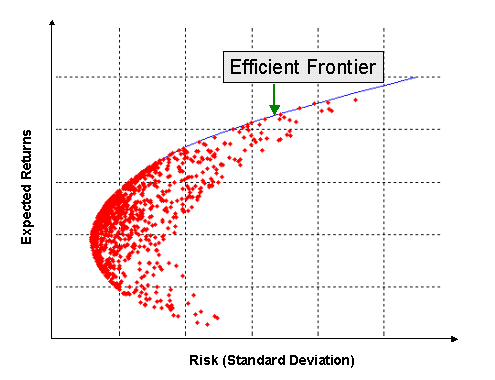
\includegraphics{Resources/efffrontier2.png}

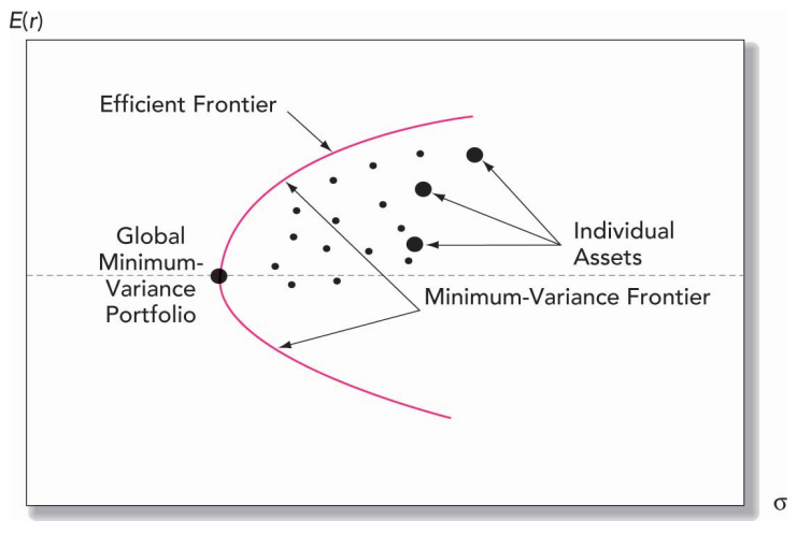
\includegraphics{Resources/efffrontier.png}

The analytical technique to derive efficient frontier was developed by Harry Markowitz, and is often referred to as the \textbf{Markowitz Model}

\hypertarget{separation-property}{%
\subsection{Separation Property}\label{separation-property}}

Separation property states that the asset allocation problem can be divided into two independent steps:

\begin{enumerate}
\def\labelenumi{\arabic{enumi}.}
\item
  Determination of the optimal risky portfolio: this portfolio will be same for all clients.
\item
  Determination of the complete portfolio that also includes the risk-free asset.
\end{enumerate}

Thus, fund managers can serve many customers by only offering at least one portfolio.

The theoretical basis of the mutual fund industry

\hypertarget{ch4}{%
\chapter{CAPM and APT}\label{ch4}}

\begin{itemize}
\tightlist
\item
  Estimate security risk premiums using capital market theory.
\item
  Construct and use the security market line (SML).
\item
  Specify and use a multifactor SML.
\item
  Use Arbitrage Pricing Theory (APT) with multiple factors to identify mis-priced securities.
\end{itemize}

\hypertarget{the-capital-asset-pricing-model-capm}{%
\section{The Capital Asset Pricing Model (CAPM)}\label{the-capital-asset-pricing-model-capm}}

The Markowitz portfolio selection model assumes all investors are rational, i.e., mean-variance optimizers.

CAPM assumes:

\begin{itemize}
\tightlist
\item
  Individual investors are price takers.
\item
  All investors have a single-period planning horizon.
\item
  No taxes or transaction costs.
\item
  Information is costless and available to all investors.
\item
  Investors interpret information identically.
\end{itemize}

\hypertarget{capm-equation}{%
\subsection{CAPM Equation}\label{capm-equation}}

\begin{itemize}
\item
  The market portfolio defines the optimal Capital Allocation Line (CAL). In theory everyone tries to reach it.
\item
  Risk premium on the market portfolio is proportional to its risk and average risk aversion.
\end{itemize}

\[
E(R_i) = R_f + \beta_i (E(R_m) - R_f)
\]

where:

\begin{itemize}
\tightlist
\item
  \(E(R_i)\) = expected return of investment
\item
  \(R_f\) = risk-free rate
\item
  \(\beta_i\) = beta of the investment
\item
  \(E(R_m) - R_f\) = market risk premium
\end{itemize}

Investors expect to be compensated for the risk and the time value of money.

For example, in NZ, BKMB is the risk free rate(note it is technically not) and additional basis point on top is the premium.

\[
E(r_M) - r_f = \bar{A} \sigma_M^2
\]

\[
E(r_i) - r_f = \beta_i [E(r_M) - r_f]
\]

Here, \(\bar{A}\) is the average level of risk aversion across investors (weighted average, by wealth).

and

\[
\beta_i = \frac{\text{cov}(r_i, r_M)}{\sigma_M^2} = \frac{\rho_{i,M} \sigma_i}{\sigma_M}
\]

The CAPM calculates the expected return of an investment by adding the risk-free rate to the \textbf{beta}-adjusted market risk premium, where beta measures the investment's sensitivity to market risk and \textbf{alpha} represents the excess return not explained by beta.

\hypertarget{security-market-line-sml}{%
\subsection{Security Market Line (SML)}\label{security-market-line-sml}}

\begin{itemize}
\tightlist
\item
  Graphs individual asset risk premiums as a function of asset risk (beta).
\item
  Provides a benchmark for evaluating portfolio performance.
\end{itemize}

\hypertarget{capm-implementation}{%
\subsection{CAPM Implementation}\label{capm-implementation}}

\begin{itemize}
\tightlist
\item
  Risk-free rate: Use short-term treasury securities.
\item
  Beta: Covariance of stock and market returns divided by market variance.
\item
  Market portfolio: Use a broad market index return.
\end{itemize}

\hypertarget{violations-and-limitations-of-the-capm}{%
\subsection{Violations and Limitations of the CAPM}\label{violations-and-limitations-of-the-capm}}

\begin{itemize}
\tightlist
\item
  Empirical tests show a weaker relation between beta and returns.
\item
  Market capitalization and book-to-market ratios predict returns better than beta.
\item
  Other anomalies include momentum effects.
\end{itemize}

\hypertarget{multifactor-models}{%
\subsection{Multifactor Models}\label{multifactor-models}}

\begin{itemize}
\tightlist
\item
  Allow for multiple systematic risk factors (e.g., GDP, inflation).
\item
  Estimate a beta for each factor using multiple regression.
\end{itemize}

Example: Fama-French Three-Factor Model

\begin{itemize}
\tightlist
\item
  Factors: Market risk, firm size, and book-to-market ratio.
\end{itemize}

\[
E(R_i) = R_f + \beta_{iM} (E(R_M) - R_f) + \beta_{iS} (E(SMB)) + \beta_{iH} (E(HML))
\]

\begin{itemize}
\tightlist
\item
  \(\beta_{iM}\), \(\beta_{iS}\), and \(\beta_{iH}\) are the betas for the market, size, and value factors.
\end{itemize}

\hypertarget{comparison-of-cml-and-sml}{%
\section{Comparison of CML and SML}\label{comparison-of-cml-and-sml}}

\begin{longtable}[]{@{}
  >{\raggedright\arraybackslash}p{(\columnwidth - 4\tabcolsep) * \real{0.1634}}
  >{\raggedright\arraybackslash}p{(\columnwidth - 4\tabcolsep) * \real{0.4183}}
  >{\raggedright\arraybackslash}p{(\columnwidth - 4\tabcolsep) * \real{0.4183}}@{}}
\toprule\noalign{}
\begin{minipage}[b]{\linewidth}\raggedright
Feature
\end{minipage} & \begin{minipage}[b]{\linewidth}\raggedright
Security Market Line (SML)
\end{minipage} & \begin{minipage}[b]{\linewidth}\raggedright
Capital Market Line (CML)
\end{minipage} \\
\midrule\noalign{}
\endhead
\bottomrule\noalign{}
\endlastfoot
\textbf{Definition} & Relationship between expected return and beta (systematic risk) & Risk-return trade-off for efficient portfolios \\
\textbf{Equation} & \(E(r_i) = r_f + \beta_i (E(r_M) - r_f)\) & \(E(r_P) = r_f + \frac{E(r_M) - r_f}{\sigma_M} \sigma_P\) \\
\textbf{Risk Measure} & Beta (systematic risk) & Standard deviation (total risk) \\
\textbf{Applicability} & Individual securities & Efficient portfolios \\
\textbf{Correct Pricing} & Securities lie on the SML & Portfolios lie on the CML \\
\textbf{Slope} & Market risk premium \((E(r_M) - r_f)\) & Sharpe ratio of the market \(\left(\frac{E(r_M) - r_f}{\sigma_M}\right)\) \\
\end{longtable}

\hypertarget{arbitrage-pricing-theory-apt}{%
\section{Arbitrage Pricing Theory (APT)}\label{arbitrage-pricing-theory-apt}}

If two portfolios are mispriced, the investor could short the high-priced portfolio and buy the low-priced portfolio.

Arbitrage opportunities last for very short periods .

\hypertarget{assumptions}{%
\subsection{Assumptions}\label{assumptions}}

\begin{itemize}
\tightlist
\item
  Returns can be described by a factor model.
\item
  \textbf{No arbitrage opportunities.}
\item
  Large number of securities to form diversified portfolios.
\end{itemize}

Like the CAPM, the APT also uses an SML for expected return and risk

\hypertarget{key-concepts}{%
\subsection{Key Concepts}\label{key-concepts}}

\begin{itemize}
\tightlist
\item
  Systematic (factor) risk remains in diversified portfolios.
\item
  Risk premium depends only on systematic risk.
\end{itemize}

\hypertarget{apt-model}{%
\subsection{APT Model}\label{apt-model}}

\textbf{Portfolio A}
Portfolio A is a well-diversified portfolio with a beta (\(\beta_P\)) of 0.7. Its excess return equation is:

\[
\begin{align}
r_P - r_f &= \alpha_P + \beta_P (r_M - r_f) \\
          &= \alpha_P + 0.7(r_M - r_f)
\end{align}
\]

\textbf{Portfolio B}
Portfolio B includes the market index and T-bills with weights of 0.7 and 0.3 respectively. Its return equation is:

\[
\begin{align}
r_p &= 0.3r_f + 0.7r_M \\
    &= r_f + 0.7(r_M - r_f)
\end{align}
\]

By shorting \$1 of Portfolio A and buying \$1 of Portfolio B, you create a zero investment, zero beta portfolio. The proceeds would be riskless.

\[
\begin{align}
\text{Proceeds} &= \text{Return from Portfolio B} - \text{Return from Portfolio A} \\
                &= r_B - r_P \\
                &= \left( r_f + 0.7(r_M - r_f) \right) - \left( r_f + \alpha_P + 0.7(r_M - r_f) \right) \\
                &= -\alpha_P
\end{align}
\]

\begin{itemize}
\tightlist
\item
  For a well-diversified portfolio \(A\):
\end{itemize}

\[
E(R_A) = R_f + \sum_{j=1}^{k} \beta_{Aj} \lambda_j
\]

\begin{itemize}
\tightlist
\item
  \(\beta_{Aj}\) is the sensitivity of portfolio \(A\) to factor \(j\).
\item
  \(\lambda_j\) is the risk premium associated with factor \(j\).
\end{itemize}

\[ \lambda_j= \beta_1 [E(r_{M1}) - r_f]\]

\hypertarget{multifactor-generalization}{%
\subsection{Multifactor Generalization}\label{multifactor-generalization}}

\begin{itemize}
\tightlist
\item
  Accommodates multiple risk factors.
\end{itemize}

\[
E(R_i) = R_f + \beta_{i1} \lambda_1 + \beta_{i2} \lambda_2 + \ldots + \beta_{ik} \lambda_k
\]

\hypertarget{apt-pros-and-cons}{%
\subsection{APT Pros and Cons}\label{apt-pros-and-cons}}

\begin{longtable}[]{@{}
  >{\raggedright\arraybackslash}p{(\columnwidth - 2\tabcolsep) * \real{0.5000}}
  >{\raggedright\arraybackslash}p{(\columnwidth - 2\tabcolsep) * \real{0.5000}}@{}}
\toprule\noalign{}
\begin{minipage}[b]{\linewidth}\raggedright
\textbf{Strengths}
\end{minipage} & \begin{minipage}[b]{\linewidth}\raggedright
\textbf{Weaknesses}
\end{minipage} \\
\midrule\noalign{}
\endhead
\bottomrule\noalign{}
\endlastfoot
reasonable description of risk and return & Complex and difficult to measure \\
Reflects various macroeconomic impacts & world of winner chicken dinner, loser loses \\
Customizable to specific markets & Requires extensive data \\
no need to measure market return directly & Dependent on accurate factor identification \\
\end{longtable}

\hypertarget{apt-v.s.-capm}{%
\subsection{APT v.s. CAPM}\label{apt-v.s.-capm}}

APT is more general in that it gets to an expected return and beta relationship without the assumption of the market portfolio

\hypertarget{ch5}{%
\chapter{Fundamental Analysis and Equity Valuation}\label{ch5}}

\hypertarget{fundamental-analysis-framework}{%
\section{Fundamental Analysis Framework}\label{fundamental-analysis-framework}}

\hypertarget{global-economic-considerations}{%
\subsection{Global Economic Considerations}\label{global-economic-considerations}}

\begin{itemize}
\tightlist
\item
  Variable performance across regions
\item
  Stock market returns did not always align with macroeconomic expectations
\item
  Political and currency risks (e.g., Brexit, exchange rate fluctuations)\texttt{{[}1{]}}
\end{itemize}

\hypertarget{domestic-macroeconomy}{%
\subsection{Domestic Macroeconomy}\label{domestic-macroeconomy}}

\begin{itemize}
\tightlist
\item
  Key economic variables: GDP, employment, inflation, interest rates
\item
  Fiscal Policy,monetary policy and its effects (e.g., budget deficits, crowding out)
\item
  Consumer sentiment and drives
\end{itemize}

Supply shocks
- policy changes
- consumer sentiment
- population change

Demand shocks
- material costs
- technology
- natural disasters, war etc

\textbf{Indicators}

\begin{itemize}
\tightlist
\item
  Leading Indicators

  \begin{itemize}
  \tightlist
  \item
    Stock prices
  \item
    Manufacturer's new orders
  \item
    Yield curve: spread between 10-year T-bond yield and federal funds rate
  \end{itemize}
\item
  Coincident

  \begin{itemize}
  \tightlist
  \item
    real-time retail sales
  \end{itemize}
\item
  Lagging

  \begin{itemize}
  \tightlist
  \item
    GDP
  \item
    unemployment rates
  \end{itemize}
\end{itemize}

\hypertarget{business-cycle}{%
\subsection{Business Cycle}\label{business-cycle}}

\textbf{Defining industry}

NAICS (North American Industry Classification System) codes

Industry classifications are never perfect

\begin{itemize}
\tightlist
\item
  Cyclical industries: high sensitivity to economic changes
\item
  Defensive industries: low sensitivity
\item
  key consideration for time series analysis
\end{itemize}

\textbf{Factors Affecting Sensitivity}:
- Sales sensitivity: Essentials vs.~non-essentials
- Operating leverage: Fixed versus variable costs
- Financial leverage: Impacts on high vs.~low financial leverage industries

\hypertarget{business-growth}{%
\subsubsection{Business Growth}\label{business-growth}}

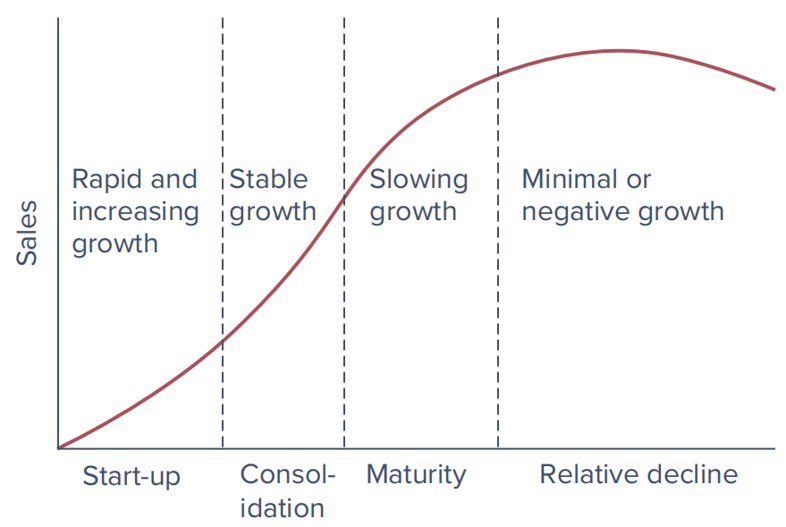
\includegraphics{Resources/businesscycle.png}

\hypertarget{lynchs-investing-categories}{%
\subsection{Lynch's Investing Categories}\label{lynchs-investing-categories}}

\begin{itemize}
\tightlist
\item
  \textbf{Slow Growers}: Large and mature companies with modest growth rates.
\item
  \textbf{Stalwarts}: Consistent and reliable performance but usually offer moderate returns.
\item
  \textbf{Fast Growers}: Characterized by rapid growth and high potential returns, these companies also carry higher risks.
\item
  \textbf{Cyclicals}: Companies whose performance is tied closely to economic cycles.
\item
  \textbf{Turnarounds}: These are companies that are currently performing poorly but have the potential for recovery.
\item
  \textbf{Asset Plays}: Companies that possess valuable assets not currently reflected in their stock price.
\end{itemize}

\textbf{Slow growers pros and cons :}

\begin{longtable}[]{@{}ll@{}}
\toprule\noalign{}
Pros & Cons \\
\midrule\noalign{}
\endhead
\bottomrule\noalign{}
\endlastfoot
Stability and Consistency & Lower Growth Potential \\
High Dividend Yield & Possible Underperformance in Bull Markets \\
Lower Risk & Limited Upside Potential \\
Predictable Performance & May Lack Excitement \\
\end{longtable}

\hypertarget{porter-19801985-determinants-of-competition}{%
\subsection{Porter (1980,1985) determinants of competition:}\label{porter-19801985-determinants-of-competition}}

\begin{itemize}
\tightlist
\item
  Threat of Entry
\item
  Rivalry between existing competitors
\item
  Pressure from substitute products
\item
  Bargaining power of buyers
\item
  Bargaining power of suppliers
\end{itemize}

\hypertarget{equity-valuation}{%
\section{Equity Valuation}\label{equity-valuation}}

\hypertarget{asset-pricing}{%
\subsection{Asset pricing}\label{asset-pricing}}

The present value (\[ P_0 \]) of an asset can be calculated using the formula:

\[ P_0 = \sum_{t=0}^{T} \frac{E(CF_t)}{(1+R_t)^t} \]

Where:

\begin{itemize}
\tightlist
\item
  \(P_0\): Present value of the asset
\item
  \(E(CF_t)\): Expected cash flow at time \(t\)
\item
  \(R_t\): Discount rate at time \(t\)
\item
  \(T\): Last period for which cash flows are considered
\end{itemize}

\hypertarget{valuation-ratios-in-finance}{%
\subsection{Valuation Ratios in Finance}\label{valuation-ratios-in-finance}}

\begin{itemize}
\tightlist
\item
  Key ratios: PE, PB, PS
\item
  Importance of comparable peer firms within industry
\end{itemize}

\textbf{P/E Ratio (Price-to-Earnings Ratio)}
- Best for mature companies with stable earnings.
- Compares a company's current share price to its earnings per share (EPS).
- Indicates how much investors are willing to pay for each dollar of earnings.

\textbf{P/B Ratio (Price-to-Book Ratio)}
- Ideal for companies with significant tangible assets, like manufacturing or real estate firms.
- Compares a company's market price per share to its book value per share.
- Book value is the net asset value of the company calculated as total assets minus total liabilities.

\textbf{P/S Ratio (Price-to-Sales Ratio)}
- Suited for high-growth companies with low or negative earnings, such as start-ups or firms in industries where profitability is not immediate.
- Compares a company's market capitalization to its total sales revenue.
- Indicates how much investors are willing to pay per dollar of sales generated by the company.

\hypertarget{pe-ratio}{%
\subsection{P/E Ratio}\label{pe-ratio}}

\begin{longtable}[]{@{}
  >{\raggedright\arraybackslash}p{(\columnwidth - 2\tabcolsep) * \real{0.2111}}
  >{\raggedright\arraybackslash}p{(\columnwidth - 2\tabcolsep) * \real{0.7889}}@{}}
\toprule\noalign{}
\begin{minipage}[b]{\linewidth}\raggedright
Factor
\end{minipage} & \begin{minipage}[b]{\linewidth}\raggedright
Influence on P/E Ratio
\end{minipage} \\
\midrule\noalign{}
\endhead
\bottomrule\noalign{}
\endlastfoot
Industry/Sector & Different industries have varying profitability and growth prospects. \\
Earnings Growth & High growth typically leads to higher P/E ratios. \\
Risk Perception & Higher risk can result in lower P/E ratios. \\
Interest Rates & Low rates often lead to higher P/E ratios. \\
Market Sentiment & Bullish sentiment can inflate P/E ratios, vice versa. \\
Company Size & Larger companies may have higher P/E ratios. \\
Dividend Policy & Regular dividends may lower P/E ratios. \\
Accounting Method & Different methods can affect reported earnings and hence P/E ratios. \\
\end{longtable}

\hypertarget{dividend-discount-model-ddm}{%
\subsection{Dividend Discount Model (DDM)}\label{dividend-discount-model-ddm}}

The DDM estimates a stock's fair value by summing the present value of its future dividends.

If the DDM value exceeds the current stock price, it suggests the stock is undervalued; if it's lower, it may be overvalued.

The Generalized Dividend Discount Model (DDM) calculates the present value of all future dividends, incorporating the discount rate and growth rate.

\[
\begin{align*}
V_0 &= \sum_{t=0}^{T} \frac{E(CF_t)}{(1+R_t)^t} \\
V_0 &= \frac{D_1}{1+k} + \frac{D_2}{(1+k)^2} + \ldots + \frac{D_H + P_H}{(1+k)^H}
\end{align*}
\]

In \textbf{perpetuity}, it simplifies to:

\[
\begin{align*}
V_0 &= \frac{D_1}{1+k} + \frac{D_2}{(1+k)^2} + \frac{D_3}{(1+k)^3} + \ldots \\
V_0 &= \frac{D_1}{k}
\end{align*}
\]

If dividends are growing at a constant rate \(g\) forever, we have the \textbf{Constant Growth Dividend Discount Model}:

\[
\begin{align*}
V_0 &= \frac{D_0 (1+g)}{1+k} + \frac{D_0 (1+g)^2}{(1+k)^2} + \frac{D_0 (1+g)^3}{(1+k)^3} + \ldots \\
V_0 &= \frac{D_1}{k-g}
\end{align*}
\]

Where:

\begin{itemize}
\tightlist
\item
  \(V_0\): Present value of the stock or asset.
\item
  \(E(CF_t)\): Expected cash flow at time \(t\), which could represent dividends, earnings, or other cash flows.
\item
  \(R_t\): Discount rate at time \(t\), often representing the required rate of return or cost of capital.
\item
  \(k\): Discount rate or required rate of return.
\item
  \(D_t\): Dividend at time \(t\).
\item
  \(P_H\): Terminal value or price at the horizon year \(H\).
\item
  \(g\): Growth rate of dividends.
\end{itemize}

\hypertarget{constant-growth-ddm}{%
\subsection{Constant Growth DDM}\label{constant-growth-ddm}}

The constant-growth Dividend Discount Model (DDM) implies that the stock price is expected to grow at the same rate as dividends.

To see this:

\[
\begin{align*}
P_1 &= \frac{D_2}{k - g} 
    = \frac{D_1 (1 + g)}{k - g} 
    = \frac{D_1}{k - g} (1 + g) \\
P_1     &= P_0 (1 + g)
\end{align*}
\]

Thus, for a stock whose market value equals intrinsic value, the expected holding period return will be:

\[
\begin{align*}
E(r) &= \text{Dividend Yield} + \text{Capital Gain Yield} \\
     &= \frac{D_1}{P_0} + \frac{P_1 - P_0}{P_0} \\
E(r) &= \frac{D_1}{P_0} + g
\end{align*}
\]
Note: we can have Various growth pattern assumptions for dividends

\hypertarget{divident-stocks}{%
\subsection{Divident stocks}\label{divident-stocks}}

\begin{longtable}[]{@{}
  >{\raggedright\arraybackslash}p{(\columnwidth - 2\tabcolsep) * \real{0.2057}}
  >{\raggedright\arraybackslash}p{(\columnwidth - 2\tabcolsep) * \real{0.7943}}@{}}
\toprule\noalign{}
\begin{minipage}[b]{\linewidth}\raggedright
Consideration
\end{minipage} & \begin{minipage}[b]{\linewidth}\raggedright
Description
\end{minipage} \\
\midrule\noalign{}
\endhead
\bottomrule\noalign{}
\endlastfoot
Preference for High Dividends & - Some investors prefer stocks with high dividends for regular income and stability. \\
& - Dividends can be attractive in volatile markets or during low-interest-rate periods. \\
Dividend Trap & - High dividend yield may signal a dividend trap if it's unsustainable due to declining earnings or cash flow. \\
& - Investing in such companies could lead to capital loss if dividends are cut. \\
Value Destruction & - Companies paying high dividends without reinvesting in growth may lead to long-term value destruction. \\
& - High dividends to support an overvalued stock could hinder future growth and harm shareholder value. \\
& \\
\end{longtable}

\hypertarget{future-earnings-ddm}{%
\subsection{future earnings DDM}\label{future-earnings-ddm}}

Rather than the earlier dividend focus, concentrates the analyst's attention on the \textbf{core business determinants of value}

Dividends = earnings - net new investment, i.e., ``\(D = E - I\)''.

\[
\begin{align}
p_0 = \sum_{t=1}^{\infty} \frac{D_t}{(1+k)^t} = \sum_{t=1}^{\infty} \frac{E_t}{(1+k)^t} - \sum_{t=1}^{\infty} \frac{I_t}{(1+k)^t}
\end{align}
\]

where:

\begin{itemize}
\tightlist
\item
  \(p_0\): Present value of the security
\item
  \(D_t\): Dividends at time \(t\)
\item
  \(E_t\): Earnings at time \(t\)
\item
  \(I_t\): Investments at time \(t\)
\item
  \(k\): Discount rate
\end{itemize}

\hypertarget{stock-valuation-scenarios}{%
\subsection{\# Stock Valuation Scenarios}\label{stock-valuation-scenarios}}

\begin{enumerate}
\def\labelenumi{\arabic{enumi}.}
\tightlist
\item
  \textbf{No Growth Scenario:}
\end{enumerate}

If all annual earnings are distributed and there is no growth

\[
   P_0 = \frac{E_1}{k}
   \]

\begin{enumerate}
\def\labelenumi{\arabic{enumi}.}
\setcounter{enumi}{1}
\item
  \textbf{Growth Opportunities Scenario:}

  If we consider the present value of growth opportunities (PVGO or NPVGO), the stock price is given by:

  \[
  P_0 = \frac{E_1}{k} + \text{NPVGO}
  \]
\item
  \textbf{Constant Growth Scenario:}

  Assuming a constant retention ratio \(b\) and a constant growth rate \(g\), the stock price can be expressed as:

  \[
  P_0 = \frac{E_1 (1 - b)}{k - g} = \frac{D_1}{k - g}
  \]
\end{enumerate}

Where:
- \(P_0\): Current stock price.
- \(E_1\): Earnings at time 1.
- \(k\): Discount rate or required rate of return.
- \(\text{NPVGO}\): Net present value of growth opportunities.
- \(b\): Retention ratio (portion of earnings retained in the company). \(g = b*ROE\).
- \(g\): Growth rate of dividends.
- \(D_1\): Dividend at time 1 (which is \(E_1 (1 - b)\)).

\hypertarget{sources-of-value-creation}{%
\subsection{Sources of Value Creation}\label{sources-of-value-creation}}

Growth stock Co.~initially has the same earnings of \$15 as No growth Co., but reinvests 60\% of its earnings each year into new investments that yield a real rate of return of 20\% per year.

\[
  \text{PV} = \frac{E_1}{k} = \frac{\$15}{0.15} = \$100
  \]

\[
  \text{PVGO} = \frac{E_1 (1 - b)}{k - g} = \frac{\$15 (1 - 0.60)}{0.15 - 0.60 \times 0.20} = \$200
  \]

However, \(g\) growth rate of dividend cannot be higher than \(k\) required rate of return or equation does not work.

\begin{Shaded}
\begin{Highlighting}[]
\NormalTok{E1 }\OtherTok{\textless{}{-}} \DecValTok{15}              \CommentTok{\# Earnings at time 1}
\NormalTok{b }\OtherTok{\textless{}{-}} \FloatTok{0.60}             \CommentTok{\# Retention ratio}
\NormalTok{k }\OtherTok{\textless{}{-}} \FloatTok{0.15}             \CommentTok{\# Discount rate or required rate of return}
\NormalTok{ROE }\OtherTok{\textless{}{-}} \FloatTok{0.20}           \CommentTok{\# Return on equity}
\NormalTok{g }\OtherTok{\textless{}{-}}\NormalTok{ b }\SpecialCharTok{*}\NormalTok{ ROE          }\CommentTok{\# Sustainable growth rate}

\CommentTok{\# Calculate stock price}
\NormalTok{P0 }\OtherTok{\textless{}{-}}\NormalTok{ (E1 }\SpecialCharTok{*}\NormalTok{ (}\DecValTok{1} \SpecialCharTok{{-}}\NormalTok{ b)) }\SpecialCharTok{/}\NormalTok{ (k }\SpecialCharTok{{-}}\NormalTok{ g)}
\NormalTok{P0}
\end{Highlighting}
\end{Shaded}

\begin{verbatim}
## [1] 200
\end{verbatim}

\begin{Shaded}
\begin{Highlighting}[]
\CommentTok{\# Calculate the PVGO}
\NormalTok{P0\_no\_growth }\OtherTok{\textless{}{-}}\NormalTok{ E1 }\SpecialCharTok{/}\NormalTok{ k}
\NormalTok{PVGO }\OtherTok{\textless{}{-}}\NormalTok{ P0 }\SpecialCharTok{{-}}\NormalTok{ P0\_no\_growth}
\NormalTok{PVGO}
\end{Highlighting}
\end{Shaded}

\begin{verbatim}
## [1] 100
\end{verbatim}

\hypertarget{pe-ratios-and-growth-scenarios}{%
\subsection{PE Ratios and Growth Scenarios}\label{pe-ratios-and-growth-scenarios}}

\textbf{No Growth Scenario}

In the no growth scenario, the stock price is given by:

\[
P_0 = \frac{E_1}{k} 
\]
Thus,

\[
\frac{P_0}{E_1} = \frac{1}{k}
\]

\textbf{constant growth scenario}

\[
\begin{aligned}
P_0 &= \frac{D_1}{k - g} \\
    &= \frac{E_1 (1 - b)}{k - b \cdot \text{ROE}}
\end{aligned}
\]

Thus,

\[
\begin{aligned}
\frac{P_0}{E_1} &= \frac{1 - b}{k - b \cdot \text{ROE}} \\
                &= \frac{1 - b}{k - g}
\end{aligned}
\]

Where:

\begin{itemize}
\tightlist
\item
  \(P_0\): Current stock price.
\item
  \(E_1\): Earnings at time 1.
\item
  \(D_1\): Dividend at time 1 (\(E_1 (1 - b)\)).
\item
  \(k\): Discount rate or required rate of return.
\item
  \(g\): Growth rate (\(b \cdot \text{ROE}\)).
\item
  \(b\): Retention ratio (portion of earnings retained in the company).
\item
  \(\text{ROE}\): Return on equity.
\end{itemize}

\hypertarget{pros-and-cons-of-a-high-pe-ratio}{%
\subsection{Pros and Cons of a High P/E Ratio}\label{pros-and-cons-of-a-high-pe-ratio}}

\begin{longtable}[]{@{}
  >{\raggedright\arraybackslash}p{(\columnwidth - 2\tabcolsep) * \real{0.5049}}
  >{\raggedright\arraybackslash}p{(\columnwidth - 2\tabcolsep) * \real{0.4951}}@{}}
\toprule\noalign{}
\begin{minipage}[b]{\linewidth}\raggedright
\textbf{Pros}
\end{minipage} & \begin{minipage}[b]{\linewidth}\raggedright
\textbf{Cons}
\end{minipage} \\
\midrule\noalign{}
\endhead
\bottomrule\noalign{}
\endlastfoot
Indicates strong growth expectations & May signal overvaluation if growth expectations are unrealistic \\
Reflects investor confidence in future performance & Higher risk if the company fails to meet growth expectations \\
Often seen in companies with innovative products or services & Can result in lower dividend yields due to reinvestment in growth \\
\end{longtable}

\hypertarget{free-cash-flow-models-firm-fcff}{%
\subsection{Free Cash Flow Models Firm FCFF}\label{free-cash-flow-models-firm-fcff}}

\[
FCFF = EBIT (1 - t_c) + \text{Depreciation} - \text{Capital Expenditures} - \text{Increase in NWC}
\]
\[
V_T = \frac{FCFF_{T+1}}{WACC - g}
\]

\[
\text{Firm Value} = \sum_{t=1}^{T} \frac{FCFF_t}{(1 + WACC)^t} + \frac{V_T}{(1 + WACC)^T}
\]

Where:

\begin{itemize}
\item
  \(EBIT\): Earnings before interest and taxes.
\item
  \(t_c\): Corporate tax rate.
\item
  \(NWC\): Net working capital.
\item
  \(WACC\): Weighted average cost of capital.
\item
  \(V_T\): Terminal value at time \(T\).
\end{itemize}

\hypertarget{free-cash-flow-models-equity-fcfe}{%
\subsection{Free Cash Flow Models Equity FCFE}\label{free-cash-flow-models-equity-fcfe}}

\[
FCFE = FCFF - \text{Interest Expense} \cdot (1 - t_c) + \text{Increases in Net Debt}
\]

\[
E_T = \frac{FCFE_{T+1}}{k_E - g}
\]

\[
\text{Intrinsic Value of Equity} = \sum_{t=1}^{T} \frac{FCFE_t}{(1 + k_E)^t} + \frac{E_T}{(1 + k_E)^T}
\]

Where:

\begin{itemize}
\tightlist
\item
  \(FCFF\): Free cash flow to the firm.
\item
  \(t_c\): Corporate tax rate.
\item
  \text{Increases in Net Debt} = \text{Principal Repayments} - \text{Proceeds from Issuance of New Debt}.
\item
  \(g\): Growth rate beyond the forecast period.
\item
  \(k_E\): Cost of equity.
\item
  \(E_T\): Terminal value at time \(T\).
\end{itemize}

\begin{Shaded}
\begin{Highlighting}[]
\CommentTok{\# Function to calculate FCFF}
\NormalTok{calculate\_fcff }\OtherTok{\textless{}{-}} \ControlFlowTok{function}\NormalTok{(EBIT, tax\_rate, depreciation, capex, delta\_nwc) \{}
\NormalTok{  fcff }\OtherTok{\textless{}{-}}\NormalTok{ EBIT }\SpecialCharTok{*}\NormalTok{ (}\DecValTok{1} \SpecialCharTok{{-}}\NormalTok{ tax\_rate) }\SpecialCharTok{+}\NormalTok{ depreciation }\SpecialCharTok{{-}}\NormalTok{ capex }\SpecialCharTok{{-}}\NormalTok{ delta\_nwc}
  \FunctionTok{return}\NormalTok{(fcff)}
\NormalTok{\}}

\CommentTok{\# Function to calculate FCFE}
\NormalTok{calculate\_fcfe }\OtherTok{\textless{}{-}} \ControlFlowTok{function}\NormalTok{(fcff, interest\_expense, tax\_rate, net\_debt\_increase) \{}
\NormalTok{  fcfe }\OtherTok{\textless{}{-}}\NormalTok{ fcff }\SpecialCharTok{{-}}\NormalTok{ interest\_expense }\SpecialCharTok{*}\NormalTok{ (}\DecValTok{1} \SpecialCharTok{{-}}\NormalTok{ tax\_rate) }\SpecialCharTok{+}\NormalTok{ net\_debt\_increase}
  \FunctionTok{return}\NormalTok{(fcfe)}
\NormalTok{\}}

\CommentTok{\# Example values}
\NormalTok{EBIT         }\OtherTok{\textless{}{-}} \DecValTok{1000000} \CommentTok{\# Earnings before interest and taxes}
\NormalTok{tax\_rate     }\OtherTok{\textless{}{-}} \FloatTok{0.30} \CommentTok{\# Corporate tax rate}
\NormalTok{depreciation }\OtherTok{\textless{}{-}} \DecValTok{200000} \CommentTok{\# Depreciation}
\NormalTok{capex        }\OtherTok{\textless{}{-}} \DecValTok{300000} \CommentTok{\# Capital expenditures}
\NormalTok{delta\_nwc    }\OtherTok{\textless{}{-}} \DecValTok{50000} \CommentTok{\# Increase in net working capital}

\CommentTok{\# Calculate FCFF}
\NormalTok{fcff }\OtherTok{\textless{}{-}} \FunctionTok{calculate\_fcff}\NormalTok{(EBIT, tax\_rate, depreciation, capex, delta\_nwc)}
\NormalTok{fcff}
\end{Highlighting}
\end{Shaded}

\begin{verbatim}
## [1] 550000
\end{verbatim}

\begin{Shaded}
\begin{Highlighting}[]
\CommentTok{\# Additional values for FCFE calculation}
\NormalTok{interest\_expense  }\OtherTok{\textless{}{-}} \DecValTok{100000} \CommentTok{\# Interest expense}
\NormalTok{net\_debt\_increase }\OtherTok{\textless{}{-}} \DecValTok{200000} \CommentTok{\# Increase in net debt}

\CommentTok{\# Calculate FCFE}
\NormalTok{fcfe }\OtherTok{\textless{}{-}} \FunctionTok{calculate\_fcfe}\NormalTok{(fcff, interest\_expense, tax\_rate, net\_debt\_increase)}
\NormalTok{fcfe}
\end{Highlighting}
\end{Shaded}

\begin{verbatim}
## [1] 680000
\end{verbatim}

\hypertarget{summary-on-valuation-models}{%
\subsection{Summary on Valuation Models:}\label{summary-on-valuation-models}}

\begin{itemize}
\tightlist
\item
  Most reliable: Market value items from balance sheet (e.g., real estate, PPE)
\item
  Less reliable: Economic profit on existing assets
\item
  Least reliable: Growth opportunities
\end{itemize}

\hypertarget{ch6}{%
\chapter{Bond Pricing and Yields}\label{ch6}}

\hypertarget{fixed-income-securities}{%
\section{Fixed Income Securities}\label{fixed-income-securities}}

\hypertarget{characteristics-of-security}{%
\subsection{characteristics of Security}\label{characteristics-of-security}}

\begin{itemize}
\tightlist
\item
  \textbf{Issuer}: The entity borrowing funds.
\item
  \textbf{Principal}: The amount borrowed.
\item
  \textbf{Coupon Rate}: Interest paid on the principal.
\item
  \textbf{Maturity}: The date when the principal is repaid.
\end{itemize}

The cash flows promised to buyers represent contractual obligations of the respective issuers.
Unlike equity securities, shareholders hold ``residual claims'' on a firm's assets.

\hypertarget{involvement}{%
\subsection{Involvement}\label{involvement}}

\begin{itemize}
\tightlist
\item
  \textbf{Issuers}

  \begin{itemize}
  \tightlist
  \item
    Different levels of governments entity
  \item
    Financial intermediaries
  \item
    Corporations
  \end{itemize}
\item
  \textbf{Investors}

  \begin{itemize}
  \tightlist
  \item
    Financial intermediaries
  \item
    Investment funds
  \item
    Superannuation funds
  \item
    Corporations
  \item
    Individuals
  \end{itemize}
\item
  \textbf{Others}

  \begin{itemize}
  \tightlist
  \item
    Credit Rating Agencies: S\&P, Moody's, Fitch
  \item
    Regulators: ASIC, APRA, SEC
  \end{itemize}
\end{itemize}

\hypertarget{bond-types}{%
\section{Bond Types}\label{bond-types}}

\begin{longtable}[]{@{}
  >{\raggedright\arraybackslash}p{(\columnwidth - 2\tabcolsep) * \real{0.2266}}
  >{\raggedright\arraybackslash}p{(\columnwidth - 2\tabcolsep) * \real{0.7734}}@{}}
\toprule\noalign{}
\begin{minipage}[b]{\linewidth}\raggedright
Bond Type
\end{minipage} & \begin{minipage}[b]{\linewidth}\raggedright
Description
\end{minipage} \\
\midrule\noalign{}
\endhead
\bottomrule\noalign{}
\endlastfoot
Fixed-Coupon Bonds & Regular interest payments and repayment of principal at maturity. \\
Indexed Bonds & Par value and coupon payments are tied to a price index, such as CPI. \\
Floating Rate Bonds & Coupon payments vary with short-term interest rates. \\
Convertible Bonds & Can be converted into a predetermined number of shares. \\
Callable and Puttable Bonds & \textbf{Callable}: Issuer can repay early. \textbf{Puttable}: Holder can demand early repayment. \\
Zero-Coupon Bonds and Others & Only pay the face value at maturity. Examples include Treasury Bills. \\
Inflation-Protected Bonds & Adjusted for inflation to protect investors from inflation risk. Example: Treasury Inflation-Protected Securities (TIPS). \\
\end{longtable}

\hypertarget{bond-prices}{%
\subsection{Bond Prices}\label{bond-prices}}

Between payment dates, interest accrues daily on the bond

\[
\text{Accrued Interest} = \text{Coupon} \times \left( \frac{\text{Days since last coupon payment}}{\text{Days between coupon payments}} \right)
\]

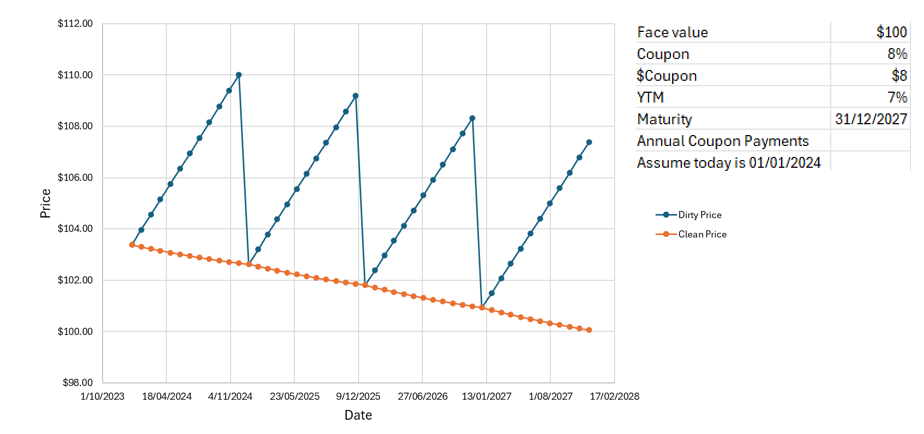
\includegraphics{Resources/bondprice.png}

The invoice price is the fair value of the bond by taking the present value of all future cash flows (clean price (or quoted price) + accrued interest)

\hypertarget{bond-yield-equations}{%
\section{Bond Yield Equations}\label{bond-yield-equations}}

\hypertarget{current-yield}{%
\subsection{Current Yield}\label{current-yield}}

\[
Current\ Yield = \frac{Annual\ Coupon\ Payment}{Current\ Market\ Price}
\]

\hypertarget{yield-to-maturity-ytm}{%
\subsection{Yield to Maturity (YTM)}\label{yield-to-maturity-ytm}}

YTM is the internal rate of return (IRR) of the bond, considering all coupon payments and the face value repayment at maturity.

It can also be interpreted as the compound rate of return over the life of the bond, assuming all coupons are reinvested at YTM

\[
P = \sum_{t=1}^{n} \frac{C}{(1+YTM)^t} + \frac{F}{(1+YTM)^n}
\]
Where:

\begin{itemize}
\tightlist
\item
  \(P\) = Current market price
\item
  \(C\) = Annual coupon payment
\item
  \(F\) = Face value of the bond
\item
  \(n\) = Number of years to maturity
\end{itemize}

\hypertarget{yield-to-call-ytc}{%
\subsection{Yield to Call (YTC)}\label{yield-to-call-ytc}}

If a bond is callable, the YTC is calculated similarly to YTM but considers the call date and call price.
\[
P = \sum_{t=1}^{t_c} \frac{C}{(1+YTC)^t} + \frac{C_p}{(1+YTC)^{t_c}}
\]
Where:

\begin{itemize}
\tightlist
\item
  \(t_c\) = Call date
\item
  \(C_p\) = Call price
\end{itemize}

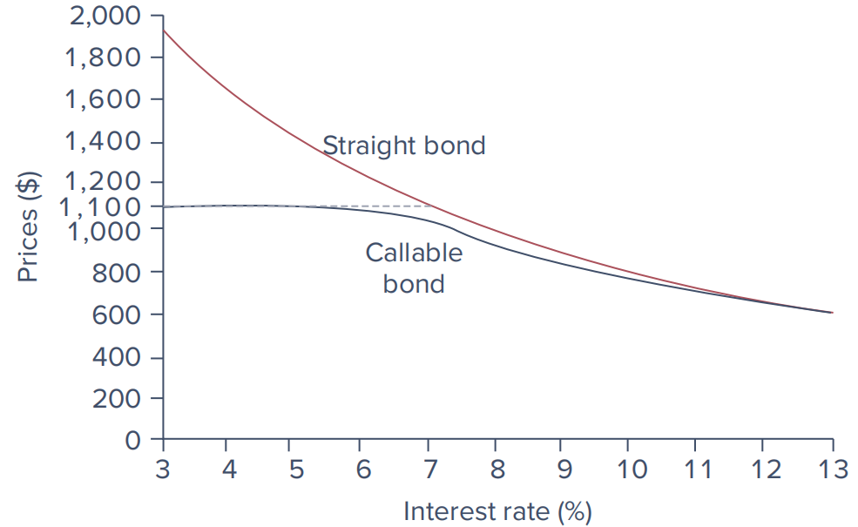
\includegraphics{Resources/callbond.png}

\hypertarget{realized-compound-return}{%
\section{Realized Compound Return}\label{realized-compound-return}}

To find the realized compound return \(r\) for investment A:

\[
1{,}000(1+r)^2 = 1{,}210
\]

Solving for \(r\):

\[
r = \left(\frac{1{,}210}{1{,}000}\right)^{\frac{1}{2}} - 1 = 0.10 \quad \text{or} \quad 10\%
\]

\begin{Shaded}
\begin{Highlighting}[]
\CommentTok{\# Variables}
\NormalTok{initial\_investment }\OtherTok{\textless{}{-}} \DecValTok{1000}
\NormalTok{final\_value }\OtherTok{\textless{}{-}} \DecValTok{1210}
\NormalTok{n }\OtherTok{\textless{}{-}} \DecValTok{2}

\CommentTok{\# Calculate and print the realized compound return}
\NormalTok{r }\OtherTok{\textless{}{-}}\NormalTok{ (final\_value }\SpecialCharTok{/}\NormalTok{ initial\_investment)}\SpecialCharTok{\^{}}\NormalTok{(}\DecValTok{1} \SpecialCharTok{/}\NormalTok{ n) }\SpecialCharTok{{-}} \DecValTok{1}
\FunctionTok{round}\NormalTok{(r }\SpecialCharTok{*} \DecValTok{100}\NormalTok{, }\DecValTok{4}\NormalTok{)}
\end{Highlighting}
\end{Shaded}

\begin{verbatim}
## [1] 10
\end{verbatim}

\hypertarget{yield-spread}{%
\subsection{Yield Spread}\label{yield-spread}}

Yield spread is the difference in yields between two different bonds, often a corporate bond and a government bond.

\[
Yield\ Spread = Yield\ of\ Corporate\ Bond - Yield\ of\ Government\ Bond
\]

\hypertarget{bond-equivalent-yield-bey}{%
\subsection{Bond Equivalent Yield (BEY)}\label{bond-equivalent-yield-bey}}

\(BEY = \frac{2 \cdot (FV - P)}{P \cdot (T)}\)

Where:
- \(FV\) = Face value
- \(P\) = Purchase price
- \(T\) = Time to maturity in years

\hypertarget{effective-annual-yield-eay}{%
\subsection{Effective Annual Yield (EAY)}\label{effective-annual-yield-eay}}

\[EAY = \left(1 + \frac{YTM}{n}\right)^n - 1\]

Where:
- \(YTM\) = Yield to maturity
- \(n\) = Number of compounding periods per year

\hypertarget{discount-yield}{%
\subsection{Discount Yield}\label{discount-yield}}

Often used for Treasury bills.
\[Discount\ Yield = \frac{(F - P)}{F} \cdot \frac{360}{Days\ to\ Maturity}\]

Where:
- \(F\) = Face value
- \(P\) = Purchase price
- \(Days\ to\ Maturity\) = Number of days until maturity

\hypertarget{bond-pricing-dynamics}{%
\section{Bond Pricing Dynamics}\label{bond-pricing-dynamics}}

\hypertarget{prices-over-time}{%
\subsection{Prices Over Time}\label{prices-over-time}}

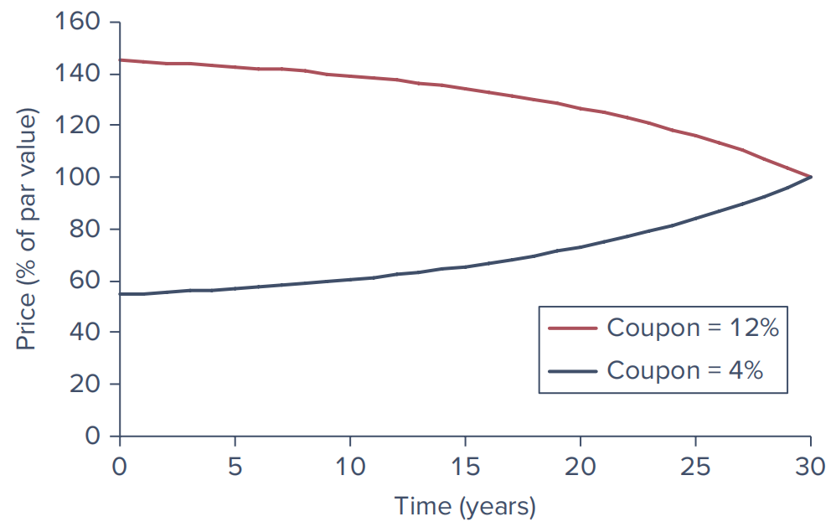
\includegraphics{Resources/parval.png}

assuming the price will shift toward par.

\begin{itemize}
\item
  \textbf{Premium Bonds}: Coupon rate exceeds YTM; price declines to par over time.
\item
  \textbf{Discount Bonds}: YTM exceeds coupon rate; price increases to par over time.
\end{itemize}

\hypertarget{holding-period-return-hpr}{%
\subsection{Holding Period Return (HPR)}\label{holding-period-return-hpr}}

\[
HPR = \frac{P_1 + (D - P_0)}{P_0}
\]
- \(P_0\): Initial price
- \(P_1\): Selling price
- \(D\): Income received (e.g., dividends)

Includes price change and income.

Useful for comparing investment performance.

\begin{Shaded}
\begin{Highlighting}[]
\CommentTok{\# Variables}
\NormalTok{P0 }\OtherTok{\textless{}{-}} \DecValTok{1000}     \CommentTok{\# Initial price}
\NormalTok{P1 }\OtherTok{\textless{}{-}} \DecValTok{1200}      \CommentTok{\# Selling price}
\NormalTok{D }\OtherTok{\textless{}{-}} \DecValTok{50}         \CommentTok{\# Dividends received}
\NormalTok{n\_years }\OtherTok{\textless{}{-}} \DecValTok{2}   \CommentTok{\# Holding period in years}

\CommentTok{\# Calculate HPR}
\NormalTok{HPR }\OtherTok{\textless{}{-}}\NormalTok{ (P1 }\SpecialCharTok{+}\NormalTok{ D }\SpecialCharTok{{-}}\NormalTok{ P0) }\SpecialCharTok{/}\NormalTok{ P0}
\NormalTok{HPR}
\end{Highlighting}
\end{Shaded}

\begin{verbatim}
## [1] 0.25
\end{verbatim}

\begin{Shaded}
\begin{Highlighting}[]
\CommentTok{\# Annualize HPR}
\NormalTok{annualized\_HPR }\OtherTok{\textless{}{-}}\NormalTok{ (}\DecValTok{1} \SpecialCharTok{+}\NormalTok{ HPR)}\SpecialCharTok{\^{}}\NormalTok{(}\DecValTok{1} \SpecialCharTok{/}\NormalTok{ n\_years) }\SpecialCharTok{{-}} \DecValTok{1}
\NormalTok{annualized\_HPR}
\end{Highlighting}
\end{Shaded}

\begin{verbatim}
## [1] 0.118034
\end{verbatim}

\hypertarget{risk-and-protection}{%
\section{Risk and Protection}\label{risk-and-protection}}

\hypertarget{default-risk}{%
\subsection{Default Risk}\label{default-risk}}

Evaluated by rating agencies like Moody's, S\&P, and Fitch.

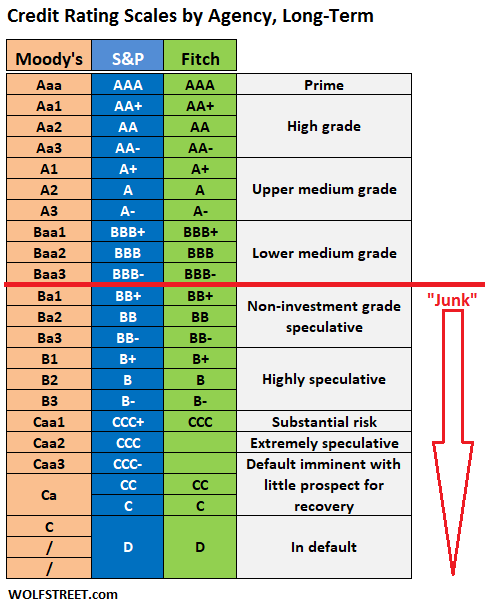
\includegraphics{creditratingsscale.png}

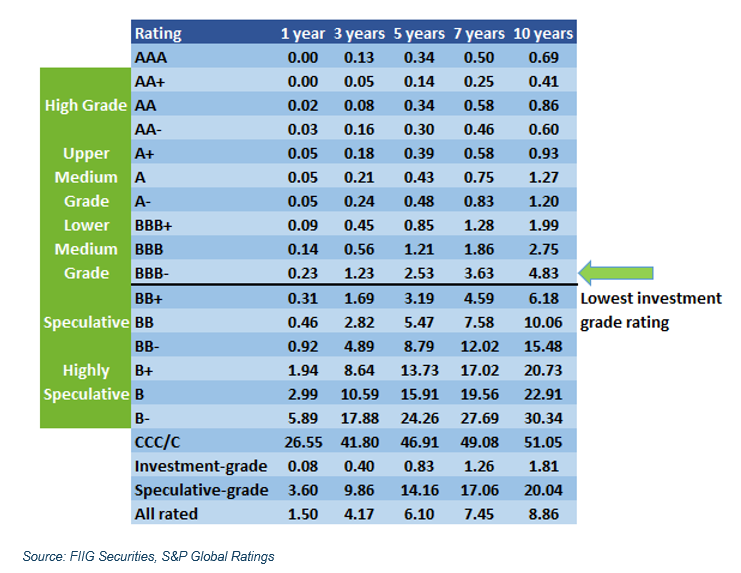
\includegraphics{quantifyingrisks.png}

\hypertarget{protection-mechanisms}{%
\subsection{Protection Mechanisms}\label{protection-mechanisms}}

\begin{itemize}
\tightlist
\item
  \textbf{Sinking Funds}: Issuer periodically repurchases bonds to reduce default risk.
\item
  \textbf{Subordination of Future Debt}: Restricts additional borrowing.
\item
  \textbf{Dividend Restrictions}: Limits on dividends to protect bondholders.
\item
  \textbf{Collateralized Bonds}: Safer than debentures.
\end{itemize}

\hypertarget{credit-default-swaps-cds}{%
\section{Credit Default Swaps (CDS)}\label{credit-default-swaps-cds}}

\begin{itemize}
\tightlist
\item
  A CDS is a contract that transfers the credit risk of a bond to another party.
\item
  \textbf{CDS Premium}: Depends on the probability of bankruptcy and the recovery rate.
\end{itemize}

\[
\begin{align}
CDS \ Premium &= (1 - Recovery \ Rate) \times Probability \ of \ Default
\end{align}
\]

\begin{itemize}
\tightlist
\item
  \textbf{Example}: A pension fund hedging default risk with a one-year CDS on a corporate bond.
\end{itemize}

\hypertarget{ch7}{%
\chapter{Enter Chapter title here}\label{ch7}}

\hypertarget{summary-of-lecture-7-fixed-income-valuation-and-term-structure}{%
\section{Summary of Lecture 7 -- Fixed Income Valuation and Term Structure}\label{summary-of-lecture-7-fixed-income-valuation-and-term-structure}}

\hypertarget{learning-objectives-1}{%
\subsection{Learning Objectives}\label{learning-objectives-1}}

\begin{itemize}
\tightlist
\item
  Understand bond pricing fundamentals and the relationship between bond prices, yield to maturity, and coupon rates.
\item
  Valuation and characteristics of zero-coupon bonds and building the yield curve.
\item
  Valuing coupon-bearing bonds using present value of future cash flows.
\item
  Factors affecting yield curve shape and deriving forward rates from the yield curve.
\end{itemize}

\hypertarget{bond-pricing-models}{%
\subsection{Bond Pricing Models}\label{bond-pricing-models}}

\hypertarget{bond-pricing-model-i}{%
\subsubsection{Bond Pricing Model I}\label{bond-pricing-model-i}}

The price of a bond is the present value of expected cash flows, including coupon and principal. The discount rate is the yield to maturity (\(YTM\)).

\[
\begin{align}
P_b &= \sum_{t=1}^{T} \frac{C_t}{(1 + r)^t} + \frac{F}{(1 + r)^T}
\end{align}
\]

\[
\text{Annualities Factor} = \frac{1}{r} \left( 1 - \frac{1}{(1 + r)^T} \right)\
\]

\[
P_B = C_t \times \text{Annuity Factor} + \text{Par} \times \text{PV Factor}\frac{C_t}{r} \left[ 1 - \frac{1}{(1 + r)^T} \right] + \frac{\text{Par}}{(1 + r)^T}
\]

Where:

\begin{itemize}
\tightlist
\item
  \(P_b\) = price of the bond
\item
  \(C_t\) = coupon payment
\item
  \(F\) = face value of the bond
\item
  \(T\) = number of periods
\item
  \(r\) is the appropriate discount rate, required return by bondholders, or yield to maturity
\end{itemize}

\begin{Shaded}
\begin{Highlighting}[]
\NormalTok{calculate\_present\_value }\OtherTok{\textless{}{-}} \ControlFlowTok{function}\NormalTok{(C\_t, r, T, Par) \{}
\NormalTok{  annuity\_factor }\OtherTok{\textless{}{-}}\NormalTok{ (}\DecValTok{1} \SpecialCharTok{{-}} \DecValTok{1} \SpecialCharTok{/}\NormalTok{ (}\DecValTok{1} \SpecialCharTok{+}\NormalTok{ r)}\SpecialCharTok{\^{}}\NormalTok{T) }\SpecialCharTok{/}\NormalTok{ r}
\NormalTok{  pv\_factor }\OtherTok{\textless{}{-}} \DecValTok{1} \SpecialCharTok{/}\NormalTok{ (}\DecValTok{1} \SpecialCharTok{+}\NormalTok{ r)}\SpecialCharTok{\^{}}\NormalTok{T}
\NormalTok{  P\_B }\OtherTok{\textless{}{-}}\NormalTok{ C\_t }\SpecialCharTok{*}\NormalTok{ annuity\_factor }\SpecialCharTok{+}\NormalTok{ Par }\SpecialCharTok{*}\NormalTok{ pv\_factor}
  \FunctionTok{return}\NormalTok{(P\_B)}
\NormalTok{\}}

\CommentTok{\# Example usage}
\NormalTok{C\_t }\OtherTok{\textless{}{-}} \DecValTok{1000}
\NormalTok{r }\OtherTok{\textless{}{-}} \FloatTok{0.05}
\NormalTok{T }\OtherTok{\textless{}{-}} \DecValTok{10}
\NormalTok{Par }\OtherTok{\textless{}{-}} \DecValTok{10000}

\NormalTok{P\_B }\OtherTok{\textless{}{-}} \FunctionTok{calculate\_present\_value}\NormalTok{(C\_t, r, T, Par)}
\NormalTok{P\_B}
\end{Highlighting}
\end{Shaded}

\begin{verbatim}
## [1] 13860.87
\end{verbatim}

\hypertarget{bond-pricing-model-ii}{%
\subsubsection{Bond Pricing Model II}\label{bond-pricing-model-ii}}

Zero-coupon bonds involve calculating the present value of the par value, discounted by the zero-coupon rate.

\[
\begin{align}
P &= \frac{F}{(1 + z_T)^T}
\end{align}
\]

\hypertarget{yield-curve}{%
\subsection{Yield Curve}\label{yield-curve}}

The yield curve plots yields-to-maturity for coupon bonds against their terms to maturity. It's crucial to understand forward rates, zero rates, and actual rates.

\hypertarget{forward-rate-calculation}{%
\subsubsection{Forward Rate Calculation}\label{forward-rate-calculation}}

Forward rates can be derived from zero rates to determine arbitrage-free pricing.

\[
\begin{align}
f_{n,n+1} &= \left( \frac{(1 + z_{n+1})^{n+1}}{(1 + z_n)^n} \right) - 1
\end{align}
\]

\hypertarget{term-structure-of-interest-rates-tsir}{%
\subsection{Term Structure of Interest Rates (TSIR)}\label{term-structure-of-interest-rates-tsir}}

TSIR describes the relationship between interest rates and terms. The yield curve can be influenced by:

\begin{enumerate}
\def\labelenumi{\arabic{enumi}.}
\tightlist
\item
  \textbf{Expectations Hypothesis}: Investors' expectations about future interest rates.
\item
  \textbf{Liquidity Preference Theory}: Prefers short-term bonds for liquidity purposes.
\item
  \textbf{Market Segmentation Theory}: Different investors have different preferred investment horizons.
\item
  \textbf{Preferred Habitat Theory}: Investors have preferred investment horizons but will deviate for adequate compensation.
\end{enumerate}

\hypertarget{valuation-of-coupon-bearing-bonds}{%
\subsection{Valuation of Coupon-Bearing Bonds}\label{valuation-of-coupon-bearing-bonds}}

To value coupon-bearing bonds, sum the present value of future cash flows (coupons and face value) discounted by the yield to maturity.

\[
\begin{align}
P &= \sum_{t=1}^{T} \frac{C}{(1 + YTM)^t} + \frac{F}{(1 + YTM)^T}
\end{align}
\]

\hypertarget{immunization}{%
\subsection{Immunization}\label{immunization}}

Immunization strategies balance exposure to interest rate movements and reinvestment risk. Duration matching is a common immunization strategy.

\[
\begin{align}
D &= \sum_{t=1}^{T} \frac{t \cdot PV(C_t)}{P}
\end{align}
\]

Where:
- \(D\) = duration
- \(PV(C_t)\) = present value of coupon at time \(t\)

\hypertarget{convexity}{%
\subsection{Convexity}\label{convexity}}

Convexity measures the sensitivity of the duration of a bond to changes in interest rates. Bonds with higher convexity are less affected by rate changes.

\[
\begin{align}
Convexity &= \sum_{t=1}^{T} \frac{t (t + 1) \cdot PV(C_t)}{(1 + YTM)^{t+2}}
\end{align}
\]

\hypertarget{conclusion}{%
\subsection{Conclusion}\label{conclusion}}

Understanding bond pricing, valuation, and the factors affecting the yield curve is crucial for fixed-income investment. Key models include the pricing of zero-coupon and coupon-bearing bonds, the yield curve, term structure theories, and strategies for immunization and duration management.

\hypertarget{ch8}{%
\chapter{Performance Attribution and Appraisal}\label{ch8}}

\hypertarget{summary-of-lecture-8-performance-attribution-and-appraisal}{%
\section{Summary of Lecture 8: Performance Attribution and Appraisal}\label{summary-of-lecture-8-performance-attribution-and-appraisal}}

\hypertarget{learning-objectives-2}{%
\subsection{Learning Objectives}\label{learning-objectives-2}}

The lecture aims to equip students with skills to:
- Compute raw and risk-adjusted rates of return.
- Evaluate investment performance.
- Apply style analysis to assess portfolio strategy.
- Decompose portfolio returns into asset allocation and security selection components.
- Assess market-timing ability.

\hypertarget{steps-in-performance-evaluation}{%
\subsection{Steps in Performance Evaluation}\label{steps-in-performance-evaluation}}

\begin{enumerate}
\def\labelenumi{\arabic{enumi}.}
\tightlist
\item
  \textbf{Performance Measurement}:

  \begin{itemize}
  \tightlist
  \item
    Calculate the return achieved by a portfolio over time.
  \end{itemize}
\item
  \textbf{Performance Appraisal}:

  \begin{itemize}
  \tightlist
  \item
    Evaluate the overall performance of the portfolio.
  \end{itemize}
\item
  \textbf{Performance Attribution}:

  \begin{itemize}
  \tightlist
  \item
    Determine the portion of performance due to the manager's skill in selecting securities.
  \end{itemize}
\end{enumerate}

\hypertarget{performance-measurement}{%
\subsection{Performance Measurement}\label{performance-measurement}}

Challenges include:
- Mismatched cash flows and measurement frequency.
- Multiple cash inflows and outflows (e.g., dividends, distributions, new funds).
- Choice of measurement methodology (Time-weighted vs.~Dollar-weighted).

\hypertarget{examples}{%
\subsubsection{Examples}\label{examples}}

\begin{itemize}
\tightlist
\item
  \textbf{Example 1 \& 2}: Calculating rate of return for one stock held over one period without dividends.
\item
  \textbf{Example 3 \& 4}: Calculating the rate of return in continuous time and with dividends.
\item
  \textbf{Example 5}: Holding one stock for multiple periods without dividends, calculating arithmetic and logarithmic rates of return.
\item
  \textbf{Example 6}: Holding one stock for multiple periods with reinvested dividends, calculating time-weighted and dollar-weighted rates of return.
\item
  \textbf{Example 7}: Managing an open-ended fund with multiple stocks, dividends, distributions, and new fund inflows, measuring time-weighted and dollar-weighted rates of return.
\end{itemize}

\hypertarget{performance-appraisal}{%
\subsection{Performance Appraisal}\label{performance-appraisal}}

The fundamental question is whether the portfolio's return of x\% is good or bad, compared to an opportunity cost with the same risk.

\hypertarget{causes-of-abnormal-performance}{%
\subsubsection{Causes of Abnormal Performance}\label{causes-of-abnormal-performance}}

\begin{itemize}
\tightlist
\item
  Asset Allocation.
\item
  Market Timing.
\item
  Security Selection.
\item
  Random influences (luck).
\end{itemize}

\hypertarget{performance-appraisal-measures}{%
\subsection{Performance Appraisal Measures}\label{performance-appraisal-measures}}

\begin{enumerate}
\def\labelenumi{\arabic{enumi}.}
\tightlist
\item
  \textbf{Simple Benchmark Index}:

  \begin{itemize}
  \tightlist
  \item
    Compare portfolio performance to a benchmark index with the same risk.
  \end{itemize}
\item
  \textbf{Sharpe Ratio}:

  \begin{itemize}
  \tightlist
  \item
    Measures excess return per unit of total risk.
  \end{itemize}
\item
  \textbf{Treynor Ratio}:

  \begin{itemize}
  \tightlist
  \item
    Measures excess return per unit of non-diversifiable risk.
  \end{itemize}
\item
  \textbf{Jensen's Alpha}:

  \begin{itemize}
  \tightlist
  \item
    Based on CAPM, measures abnormal performance.
  \end{itemize}
\item
  \textbf{Information Ratio}:

  \begin{itemize}
  \tightlist
  \item
    Measures abnormal return per unit of risk (active return-to-risk ratio).
  \end{itemize}
\item
  \textbf{M\^{}2 Measure}:

  \begin{itemize}
  \tightlist
  \item
    Compares a new portfolio combining P and the risk-free asset to the market portfolio.
  \end{itemize}
\end{enumerate}

\hypertarget{conclusion-1}{%
\subsection{Conclusion}\label{conclusion-1}}

Effective performance appraisal requires understanding and utilizing various metrics and methods to evaluate and attribute portfolio performance accurately, considering both risk and return\texttt{{[}1{]}}.

\hypertarget{ch9}{%
\chapter{Tax Implications and ESG Investing}\label{ch9}}

\hypertarget{enter-subsection-1-here}{%
\section{Enter subsection 1 here}\label{enter-subsection-1-here}}

\hypertarget{enter-subsection-2-here}{%
\section{Enter subsection 2 here}\label{enter-subsection-2-here}}

\hypertarget{concluding-remarks}{%
\chapter*{Concluding Remarks}\label{concluding-remarks}}
\addcontentsline{toc}{chapter}{Concluding Remarks}

\hypertarget{three-points-learnt}{%
\section*{Three points learnt}\label{three-points-learnt}}
\addcontentsline{toc}{section}{Three points learnt}

Summarise three major point that you learnt from this course:

\begin{itemize}
\tightlist
\item
\item
\item
\end{itemize}

\hypertarget{three-questions-to-ask}{%
\section*{Three questions to ask}\label{three-questions-to-ask}}
\addcontentsline{toc}{section}{Three questions to ask}

Come up with three questions to ponder:

\begin{itemize}
\tightlist
\item
\item
\item
\end{itemize}

\hypertarget{remarks}{%
\section*{Remarks}\label{remarks}}
\addcontentsline{toc}{section}{Remarks}

\begin{itemize}
\tightlist
\item
\end{itemize}

\hypertarget{how-to-use-rbookdown}{%
\chapter*{How to use RBookDown}\label{how-to-use-rbookdown}}
\addcontentsline{toc}{chapter}{How to use RBookDown}

Firstly, you will have to read the \href{https://bookdown.org/yihui/bookdown/}{RBookDown Bible} by YiHui Xie

In essence, you write in a mixture of markdown (For basics), html (to extend on markdown) and latex language (mostly for equations) to create a simple Note.

You can customise your style and theme through your own CSS.

RMarkdown are mostly used to knit e-books(HTML), use TexStudio if you want a proper PDF, it is easier.

\textbf{Here are some useful tips to get started}

1: To add a chapter, just open a R file and save as \texttt{.RMD}. Use number 0 to 99 with a hyphen \texttt{-} to order the RMD files and maybe add a Chapter name so it is easier to select from \texttt{Files} window at bottom right of the R Studio.

2: Code chunks can generate graphical outputs, To insert pictures just use \texttt{include\_graphics} instead of \texttt{\textbackslash{}includegraphics\{\}} or \texttt{!{[}{]}()}. Width can be customised.

\begin{verbatim}
knitr::include_graphics(rep('images/knit-logo.png', 3))
\end{verbatim}

3: Use 1 grave accent ` to include the in line code, use 3 grave accent to include a chunk of code.

  \bibliography{references.bib}

\end{document}
